\documentclass{article}
\usepackage{setspace}
%\usepackage{subfigure}

\pagestyle{plain}
\usepackage{amssymb,graphicx,color}
\usepackage{amsfonts}
\usepackage{latexsym}
\usepackage{a4wide}
\usepackage{amsmath}
\usepackage{paper}
\usepackage{mathtools}
\usepackage{algorithm}
\usepackage{algpseudocode}
\usepackage{cfr-lm}
\usepackage{sectsty}
\usepackage{pgf -umlcd}
\usepackage{xcolor}
\usepackage{listings}
\definecolor{light-gray}{gray}{0.95}
\lstdefinestyle{yaml}{
     backgroundcolor=\color{light-gray},
     numbers=left,
     showstringspaces=true,
     basicstyle=\color{black}\scriptsize,
     rulecolor=\color{black},
     string=[s]{'}{'},
     stringstyle=\color{black},
     comment=[l]{:},
     commentstyle=\color{blue},
     morecomment=[l]{-}
 }

% \sectionfont{\fontsize{12}{12}\selectfont}
% \subsectionfont{\fontsize{11}{11}\selectfont}
% \subsectionfont{\fontsize{10}{10}\selectfont}
\newtheorem{theorem}{Theorem}
\newtheorem{lemma}[theorem]{Lemma}
\newtheorem{corollary}[theorem]{Corollary}
\newtheorem{proposition}[theorem]{Proposition}
\newtheorem{remark}[theorem]{Remark}
\newtheorem{definition}[theorem]{Definition}
\newtheorem{fact}[theorem]{Fact}

\newtheorem{problem}[theorem]{Problem}
\newtheorem{exercise}[theorem]{Exercise}
\def \set#1{\{#1\} }
\sectionfont{\fontsize{12}{12}\selectfont}
\subsectionfont{\fontsize{11}{11}\selectfont}
\subsubsectionfont{\fontsize{10}{10}\selectfont}
\def\code#1{\texttt{#1}}
\usepackage[nottoc,notlot,notlof]{tocbibind}




\newenvironment{proof}{
PROOF:
\begin{quotation}}{
$\Box$ \end{quotation}}

\usepackage{xcolor}
\newcommand{\jk}[1]{{\color{blue} [JK: #1]}}
\newcommand{\jw}[1]{{\color{gray} [JW: #1]}}
\newcommand{\vw}[1]{{\color{green} [VW: #1]}}

\newcommand{\calF}{\boldsymbol{\mathcal{F}}}
\newcommand{\bbP}{\mathbb{P}}
\newcommand{\bbR}{\mathbb{R}}
\newcommand{\bbD}{\mathbb{D}}
\newcommand{\bbN}{\mathbb{N}}
\newcommand{\bbE}{\mathbb{E}}
\newcommand{\bbV}{\mathbb{V}}
\newcommand{\bbQ}{\mathbb{Q}}
\newcommand{\bbC}{\mathbb{C}}
\newcommand{\calX}{\mathcal{X}}
\newcommand{\calY}{\mathcal{Y}}
\newcommand{\calZ}{\mathcal{Z}}
\newcommand{\calB}{\mathcal{B}}
\newcommand{\calP}{\mathcal{P}}
\newcommand{\calQ}{\mathcal{Q}}
\newcommand{\calS}{\mathcal{S}}
\newcommand{\calN}{\mathcal{N}}
\newcommand{\calO}{\mathcal{O}}
\newcommand{\calM}{\mathcal{M}}
\newcommand{\KL}{\operatorname{KL}}
\newcommand{\MMD}{\operatorname{MMD}}
\newcommand{\JSD}{\operatorname{JSD}}



\newcommand{\nats}{\mbox{\( \mathbb N \)}}
\newcommand{\rat}{\mbox{\(\mathbb Q\)}}
\newcommand{\rats}{\mbox{\(\mathbb Q\)}}
\newcommand{\reals}{\mbox{\(\mathbb R\)}}
\newcommand{\ints}{\mbox{\(\mathbb Z\)}}
\newcommand{\Cat}{\operatorname{\mathcal{C}}}
\newcommand{\Chol}{\operatorname{Chol}}
\newcommand{\KLD}{\operatorname{\mathbb{KL}}}
\newcommand{\D}{\operatorname{\mathbb{D}}}
\newcommand{\WD}{\operatorname{\mathbb{W}_2}}
\newcommand{\tr}{\operatorname{tr}}
\newcommand{\diag}{\operatorname{diag}}
\newcommand{\GP}{\operatorname{\mathcal{GP}}}
\newcommand{\wc}{\operatorname{{}\cdot{}}}

\DeclareMathOperator*{\argmax}{arg\,max}
\DeclareMathOperator*{\argmin}{arg\,min}

% make sure equation numbers start with the section they are from
\numberwithin{equation}{section}
%%%%%%%%%%%%%%%%%%%%%%%%%%


\begin{document}

\onehalfspacing
\begin{titlepage}
	\centering
\begin{figure}[h!]
\begin{flushright}
    
\includegraphics[width=.333\textwidth]{ucl_logo.png}
\end{flushright}
\end{figure}
    {}
	\vspace{4.5cm}

	{\Huge\bfseries Generalised Variational Inference \\ for Gaussian Processes\par}
	% \vfill

	\vspace{1cm}
	{\Large\itshape James Wu\par}
	\vspace{0.5cm}
	supervised by\par
	\vspace{0.25cm}
    Veit D. \textsc{Wild} \& Jeremias \textsc{Knoblauch}
	\vfill
	{\large September 2023\par}
	\vspace{2cm}
	% \vfill

% Bottom of the page
\end{titlepage}
\pagenumbering{gobble}
\newpage
\setcounter{page}{1}
\pagenumbering{roman}

This report is submitted as part requirement for the Master's in Computational Statistics \& Machine Learning Degree at University College London (UCL). It is substantially the result of my own work except where explicitly indicated in the text.

\begin{flushright}
    \textit{James (Jian Shu) Wu}

    September 2023
\end{flushright}
\newpage


\section*{Acknowledgements}
Thanks mom!
\newpage

\begin{abstract}
Summarise your report concisely.
\end{abstract}
\newpage
\tableofcontents
\newpage
\pagenumbering{arabic}
\setcounter{page}{1}
\counterwithin{figure}{section}
\setcounter{section}{-1}
\section{Notation}
We begin with some general remarks on the notation used in the following sections. 
We will denote $\mathcal{X}$ as any input space, $\mathbb{R}$ as the real space, $\mathbb{R}^N$ as an $N$-dimensional real space, and $\{\cdots\}$ as a space constructed by a custom set of elements. The bolded letters $\boldsymbol{\boldsymbol{\mathcal{F}}}$, $\boldsymbol{\mathcal{G}}$, $\boldsymbol{\mathcal{Q}}$, and $\boldsymbol{\Gamma}$ will also denote spaces and will be defined when used.

A Gaussian distribution will be denoted $\mathcal{N}(\cdot, \cdot)$ where 
\begin{align}
    Y \sim \mathcal{N}(\mathbf{m}, \mathbf{K}),
\end{align}
such that $Y \in \mathbb{R}^N$ denotes that $Y$ is an $N$ dimensional random vector taking values in $\mathbb{R}^N$ following a Gaussian distribution with $\mathbf{m} \in \mathbb{R}^N$ as the mean vector and $\mathbf{K} \in \mathbb{R}^{N \times N}_{\succcurlyeq 0}$ as the covariance matrix. 
The notation $\mathbf{K} \in \mathbb{R}^{N \times N}_{\succcurlyeq 0}$ indicates that $\mathbf{K}$ is a real-valued matrix of shape $N \times N$ that is positive semi-definite, which is denoted by the subscript ${\succcurlyeq 0}$. 


For any random element $F$ taking values in some space $\boldsymbol{\boldsymbol{\mathcal{F}}}$, we review the three notational conventions:
\begin{enumerate}
    \item sample notation: 
        \begin{align}
            F \sim \mathcal{N}(\cdot, \cdot),
        \end{align}
        and becomes $F \vert Y$ when conditioned on $Y$,
    \item measure notation: 
        \begin{align}
            \mathbb{P}^F = \mathcal{N}(\cdot, \cdot),
        \end{align}
        where $\mathbb{P}^F$ is the probability measure of $F$ or alternatively $\mathbb{P}(F) = \mathcal{N}(\cdot, \cdot)$, and when conditioned becomes $\mathbb{P}(F \vert Y)$, and
    \item probability density notation: 
        \begin{align}
           p(f) = \mathcal{N}(\cdot, \cdot),
        \end{align}
        when there exists a density $p$ with respect to some other measure, most commonly the Lebesgue measure. When conditioned on $Y$, we denote $p(f\vert Y)$.
\end{enumerate}
Sample, measure, and probability density notation will be used interchangeably whenever appropriate. We will also define new notation such as $P \coloneqq \mathbb{P}(F)$ and $Q \coloneqq \mathbb{Q}(F)$ whenever convenient. $\mathbb{E}_{P}[\wc]$ denotes expectation with respect to $P$ and $\mathbb{D}[Q, P]$ denotes a divergence between the measures $Q$ and $P$. Other divergences will follow similar notation and will be defined whenever needed.

\newpage
\section{Gaussian Processes}\label{section:gaussian-processes}
Gaussian processes (GPs) are powerful universal function approximators that can be used for both regression and classification tasks. We will introduce the GP following \cite{rasmussen2003gaussian}, \cite{matthews2017scalable}, and \cite{wild2022generalized}.

\subsection{The Gaussian Process}\label{section:the-gp}
A Gaussian process (GP) is a stochastic process such that for any $N$ points $\mathbf{X} \coloneqq \left\{ x_n\right\}_{n=1}^N$ where $x_n \in \mathcal{X}$, the corresponding random response vector $Y \in \mathbb{R}^N$ has the Gaussian distribution
\begin{align}
    \label{gp-vector}
    Y \sim \mathcal{N}\left(\mathbf{m}, \mathbf{K}\right),
\end{align}
where $\mathbf{m} \in \mathbb{R}^N$ and $\mathbf{K} \in  \mathbb{R}^{N \times N}_{\succcurlyeq 0}$.
The mean vector $\mathbf{m}$ is constructed through the selection of a mean function mapping $m: \mathcal{X} \rightarrow \mathbb{R}$ such that
\begin{align}
    \label{gp-mean-vector}
    \mathbf{m} \coloneqq \left[ m(x_1) \cdots m(x_N)\right]^T,
\end{align}
while constructing $\mathbf{K}$ involves choosing a kernel function mapping $k: \mathcal{X} \times \mathcal{X} \rightarrow \mathbb{R}$ such that each element of the matrix is the evaluation
\begin{align}
    \label{gp-kernel-matrix}
    \left[\mathbf{K}\right]_{n, n'} \coloneqq k(x_n, x_{n'}),
\end{align}
for $n, n'=1,\dots, N$.
$\mathbf{K}$ is also known as the gram matrix.
Appendix \ref{appendix:positive-definite-kernel} shows that choosing kernel functions defined as inner products of a feature space mapping will ensure that $\mathbf{K}$ is positive semi-definite for a valid covariance matrix.


The distribution in (\ref{gp-vector}) is a finite-dimensional instance of the GP random function mapping
\begin{align}
    F \sim \GP(m, k),
    \label{gp}
\end{align}
 where $F \coloneqq \left\{F(x): x \in \mathcal{X}\right\}$ such that a sample path from $F$ has the mapping $f: \mathcal{X} \rightarrow \mathbb{R}$.
In other words, choosing a mean and kernel to construct (\ref{gp}) ensures that \textit{any} finite set of inputs will have a consistent joint Gaussian distribution adhering to (\ref{gp-vector}).

GPs are a powerful modelling approach. With minimal restrictions for choosing the mean function and kernel function, there are endless possibilities for constructing expressive GP model spaces.
This control and visibility into the model's behaviour is a strong advantage of GPs compared to other approaches.

\cite{novak2019neural} explains that the GP is an important construction for understanding the theoretical properties of many neural network architectures at initialisation.
Showing that the infinite width limit of many such architectures can be expressed as a GP has provided a theoretical framework for analysing neural networks typically viewed as black box approaches.
This provides further motivation for the potential and importance of GPs.

\subsection{Gaussian Process Regression}
Consider the regression task where we have $N$ observation pairs $(\mathbf{X}, \mathbf{Y}) \coloneqq \left\{(x_n, y_n)\right\}_{n=1}^{N}$ with inputs $x_n \in \mathcal{X}$ and responses $y_n \in \mathbb{R}$. GP regression models the data generating process as
\begin{align}
    y \sim F(x) + \epsilon,
    \label{regression-data-uncertainties}
\end{align}
where the GP random function mapping $F$ accounts for the epistemic (model) uncertainty and the random scalar $\epsilon$ accounts for the aleatoric (measurement) uncertainty. In this formulation, we assume that the aleatoric uncertainty is homoscedastic of the form
\begin{align}
    \epsilon \sim \mathcal{N} \left(0, \sigma^2\right).
    \label{aleotric-uncertainty}
\end{align}

In GP regression, the Bayesian posterior for a test point $x \in \mathcal{X}$ when conditioned on training data $\mathbf{X}$ and $\mathbf{Y}$, acts as a `prediction' for the epistemic uncertainty of the test data responses. With all terms being Gaussian, this posterior has a closed-form conditional Gaussian expression.
Having also chosen the aleoteric data uncertainty to be modelled as Gaussian in (\ref{aleotric-uncertainty}), GP regression models the test data response $y \in \mathbb{R}$ as
\begin{align}
    y \vert \mathbf{X}, \mathbf{Y}, \sigma^2
    \sim \mathcal{N}\left(\bar{m}(x), \bar{k}(x, x)\right),
    \label{gp-posterior-normal}
\end{align}
with
\begin{align}
    \label{gp-posterior-mean}
    \bar{m}(x) = m(x) + \mathbf{K}_{x, \mathbf{X}} \left(\mathbf{K}_{\mathbf{X}, \mathbf{X}} + \sigma^2 \mathbf{I}\right)^{-1} \left( \mathbf{Y} - \mathbf{m}_{\mathbf{X}}\right),
\end{align}
and
\begin{align}
    \label{gp-posterior-covariance}
    \bar{k}(x, x) = k(x, x) - \mathbf{K}_{x, \mathbf{X}} \left(\mathbf{K}_{\mathbf{X}, \mathbf{X}} + \sigma^2 \mathbf{I}\right)^{-1} \mathbf{K}_{\mathbf{X}, x},
\end{align}
where $\mathbf{m}_{\mathbf{X}}$ is more verbose notation for (\ref{gp-mean-vector}), $\mathbf{K}_{\mathbf{X}, \mathbf{X}}$ is verbose for (\ref{gp-kernel-matrix}), $\mathbf{K}_{x, \mathbf{X}} \in \mathbb{R}^{1 \times N}$ and $\mathbf{K}_{\mathbf{X}, x} \in \mathbb{R}^{N \times 1}$ are gram matrices constructed with $\mathbf{X}$ and $x$ following (\ref{gp-kernel-matrix}), and $\mathbf{I} \in \mathbb{R}^{N \times N}$ is the identity matrix.

\subsection{Gaussian Process Classification}
Consider the classification task where we have $N$ observation pairs $(\mathbf{X}, \mathbf{Y}) \coloneqq \left\{(x_n, y_n)\right\}_{n=1}^{N}$ with inputs $x_n \in \mathcal{X}$ and label responses $y_n \in \{1, \dots, J\}$. In other words, we wish to map each input $x_n$ to one of $J$ labels. Following the approach from \cite{matthews2017scalable}, GPs can be used for classification through the model
\begin{align}
    Y \sim \mathcal{C}\Big(s\left(F_1(x), \dots, F_J(x)\right)\Big),
    \label{gp-classifier}
\end{align}
where we construct GPs $F_j \sim \GP\left(m_j, k_j\right)$ for each label $j=1, \dots J$, such that $F_1, \dots, F_J$ are stochastically independent GPs and $s: \mathbb{R}^J \rightarrow \Delta(J)$ is a mapping to a $J$ dimensional probability simplex parameterising a categorical distribution $\mathcal{C}$ (a generalisation of the Bernoulli distribution to $J$ labels). In other words, the probability of the $j^{th}$ label is
\begin{align}
    \mathbb{P}(Y=j) = s_j(F_1(x), \dots, F_J(x)),
\end{align}
the $j^{th}$ element of the probability simplex $s(\cdot)$.

\cite{matthews2017scalable} provides a few different choices for $s$ in (\ref{gp-classifier}). We follow \cite{wild2022generalized}, using the robust max function to define the $j^{th}$ element of the probability simplex with
\begin{align}
s_{j}\left(f_1, \dots, f_J\right) = \begin{cases}
      1-\delta, &  \text{if } j = \argmax_{j=1\dots J}\left(f_j\right), \\
      \frac{\delta}{J-1}, & \text{otherwise}, \\
   \end{cases}
   \label{robust-max-function}
\end{align}
where $\delta \in [0, 1]$. Typically, $\delta$ is chosen as a very small value (i.e. $1e^{-2}$). Constructing the $\Delta(J)$ vector with (\ref{robust-max-function}), we have the probability value of $1-\delta$ for the label of maximum value and $\frac{\delta}{J-1}$ otherwise. This formulation provides robustness to outliers, as it only considers the ranking of the GP models for each label.

A benefit of the robust max function is that the expected log-likelihood under the categorical distribution in (\ref{gp-classifier}) becomes analytically tractable. \cite{wild2022generalized} shows that with $N$ input and response pairs, the expected log-likelihood is
\begin{align}
    \mathbb{E} \left[\log p\left(y \vert x\right)\right] \approx \sum_{n=1}^N \log(1-\epsilon) S(x_n, y_n) + \log\left(\frac{\epsilon}{J-1}\right) \left(1-S(x_n, y_n)\right),
    \label{robust-max-function-expected-log-likelihood}
\end{align}
with
\begin{align}
    S(x, j) \coloneqq \frac{1}{\sqrt{\pi}}\sum_{i=1}^{I} w_i \left(\prod_{j'=1, j'\neq j}^J \phi\left(\frac{\xi_i\sqrt{(2 k_{j'}(x, x)}+m_j(x) - m_{j'}(x)}{\sqrt{k_{j'}(x, x)}}\right)\right)
\end{align}
and $\left\{w_i, \xi_i\right\}_{i=1}^I$ are respectively the weights and roots of the Hermite polynomial of order $I \in \mathbb{N}$. $\phi(\cdot)$ is the standard normal cumulative distribution function.

\newpage
\section{Variational Inference for Gaussian Processes}\label{section:vi-gp}
A major drawback of GPs has been their inability to scale with respect to $N$, the number of training points.
Both classification and regression predictive posteriors rely on evaluating the inversion of an $\mathbb{R}^{N \times N}$ matrix in (\ref{gp-posterior-mean}) and (\ref{gp-posterior-covariance}).
This operation has computational complexity $\mathcal{O}(N^3)$ and space complexity $\mathcal{O}(N^2)$, both of which quickly become problematic when scaling to larger-sized training sets.
Despite their impressive performance and theoretically-driven approach, the computational intractability of GPs has been a serious limitation, restricting their use to problem domains having smaller sized data sets.
In this section, we will review Variational Inference (VI) for GPs to obtain computationally cheaper approximations of the true predictive posterior.
We will also discuss the challenges of learning within this framework.

\subsection{Variational Inference in Finite Dimensions}\label{section:vi-in-finite-dimensions}
Although GPs are objects constructed in an infinite dimensional setting, this section will first review VI in a finite dimensional setting.

A Bayesian approach to modelling begins with assuming a data generating process for an observation $y$ as conditionally dependent on $M$ unobserved latent random variables $Z$ through a likelihood $p(Y=y\vert Z)$ and a prior on the latent variables $p(Z)$.
These are used for the Bayesian posterior \vw{here you need to use the pdfs i.e. $p(Z|Y=y)$ and $p(z)$. The formula looks different if you write it for measures.}\jw{done, thanks.}
\begin{align}
    p(Z \vert Y=y) \propto p(Y=y\vert Z)p(Z),
    \label{bayesian-posterior}
\end{align}
which is often computationally and/or analytically intractable.
This has motivated the need for variational methods like VI to approximate (\ref{bayesian-posterior}).
VI is based on the observation that the Kullback-Leibler (KL) divergence between an arbitrary probability measure $Q \coloneqq \mathbb{Q}(Z)$ and the true Bayesian posterior $\mathbb{P}(Z\vert Y)$ can be rewritten as
\begin{align}
    \KLD\left[Q, \mathbb{P}(Z \vert Y)\right] = L(Q) - \log p(y),
    \label{finite-dimensional-vi-kld}
\end{align}
where
\begin{align}
    L(Q) \coloneqq -\mathbb{E}_{Q}\left[\log p(y \vert Z)\right] + \KLD(Q, P),
    \label{finite-dimensional-vi-loss}
\end{align}
having $P \coloneqq \mathbb{P}(Z)$ the prior, $p(y) = \int p(y\vert z)p(z) dz$ the marginal log-likelihood, $\mathbb{E}_{Q}\left[\wc \right]$ denoting the expectation with respect to $Q$, and $\KLD\left[\wc, \wc\right]$ denoting the KL divergence.
It follows that
\begin{align}
    \argmin_{Q \in \boldsymbol{Q}} \KLD\left[Q, \mathbb{P}(Z\vert Y)\right] = \argmin_{Q \in \boldsymbol{Q}} L(Q),
    \label{optimal-approximation-vi}
\end{align}
where $\boldsymbol{Q}$ is a set of candidate probability measures.
In other words, approximating the posterior by minimising (\ref{finite-dimensional-vi-kld}) is equivalent to minimising (\ref{finite-dimensional-vi-loss}). Typically, $\boldsymbol{Q}$ is constructed with respect to a parameter set $\boldsymbol{\Gamma}$ such that
\begin{align}
    \boldsymbol{Q} \coloneqq \left\{Q_{\gamma}: \gamma \in \boldsymbol{\Gamma} \right\},
\end{align}
where $\boldsymbol{\Gamma}$ is a euclidean parameter space such that solving
\begin{align}
    \gamma^* \in \argmin_{\gamma \in \boldsymbol{\Gamma}} L(Q_{\gamma})
\end{align}
obtains $Q_{\gamma^*}$ the VI approximation of the Bayesian posterior minimising (\ref{finite-dimensional-vi-kld}). The VI procedure depends on three important assumptions to ensure a reasonable approximation:
\begin{enumerate}
    \item the parameterised set of measures $\boldsymbol{Q}$ is large enough to contain a reasonable approximation of the true Bayesian posterior,
    \item the parameterisation of $Q$ ensures that $L(Q)$ is tractable or easy to approximate, and
    \item there exists an optimisation procedure that can find a reasonable minimiser $\gamma^*$.
\end{enumerate}
These three assumptions are in tension with each other.
For example, a larger approximation space $\boldsymbol{Q}$ can cause $L(Q)$ to be intractable or create a more difficult optimisation setup.
However in practice, VI can be quite successful if employed by well-informed practitioners.

\subsection{Sparse Variatonal Gaussian Processes}\label{section:svgp}
\jw{is it sparse or stochastic variational GP? lol}
To overcome the computationally intractable GP we review \cite{titsias2009variational}, which proposed the variational approximation for the Bayesian predictive posterior in (\ref{gp-posterior-normal}) as
\begin{align}
    \mathbb{Q}(F) \coloneqq \GP(m_Q, r),
\end{align}
where the mean function is
\begin{align}
    \label{svgp-mean}
    m_Q(x) = m_P(x) + \mathbf{K}_{x, \mathbf{Z}}\left(\mathbf{K}_{\mathbf{Z}, \mathbf{Z}}\right)^{-1} \boldsymbol{\mu}
\end{align}
and the kernel function is
\begin{align}
r(x, x) = k(x, x) - \mathbf{K}_{x, \mathbf{Z}}\left(\mathbf{K}_{\mathbf{Z}, \mathbf{Z}}\right)^{-1} \mathbf{K}_{\mathbf{Z}, x} + \mathbf{K}_{x, \mathbf{Z}}\left(\mathbf{K}_{\mathbf{Z}, \mathbf{Z}}\right)^{-1}\mathbf{\Sigma}\left(\mathbf{K}_{\mathbf{Z}, \mathbf{Z}}\right)^{-1} \mathbf{K}_{\mathbf{Z}, x}.
\label{svgp-covariance}
\end{align}
This defines a parameter space
\begin{align}
    \mathbf{\Gamma} = \left\{\boldsymbol{\mu} \in \mathbb{R}^{M}, \mathbf{\Sigma} \in \mathbb{R}^{M\times M}_{\succcurlyeq 0}, \mathbf{Z} \in \mathcal{X}^M \right\},
    \label{svgp-parameter-space}
\end{align}
where $m_P$ and $k$ are the mean and kernel functions of the target GP that we want to approximate. $\mathbf{Z}$ is $M$ inducing points, typically chosen as some subset of $\mathbf{X}$.
Following (\ref{finite-dimensional-vi-loss}), the variational loss for a candidate $Q \coloneqq \mathbb{Q}(F)$ becomes
\begin{align}
L(Q) = -\sum_{n-1}^N \mathbb{E}_Q \left[\log p(y_n \vert F(x_n)\right] + \KLD\left[\mathbb{Q}^F, \mathbb{P}^F\right],
\label{svgp-vi-loss}
\end{align}
where the expectation in (\ref{svgp-vi-loss}) is tractable, since $F(x_n)$ is Gaussian under $Q$.
However it is unclear if the KL divergence between two GPs in the second term is even well-defined and from a practical viewpoint, computable.
\cite{matthews2016sparse} points out that the choice of $m_Q$ and $r$ by \cite{titsias2009variational} ensures that
\begin{align}
    \KLD\left[\GP\left(m_Q, r\right), \GP\left(m_P, k\right)\right] = \KLD\left[\mathcal{N}\left(\boldsymbol{\mu}, \mathbf{\Sigma}\right), \mathcal{N}\left(\mathbf{m}_{\mathbf{Z}}, \mathbf{K}_{\mathbf{Z}, \mathbf{Z}}\right)\right],
\end{align}
reducing the KL divergence between two stochastic processes to
\begin{align}
        \KLD\left[\mathbb{Q}^F, \mathbb{P}^F\right]
    = \frac{1}{2}\left( \tr\left(\left(\mathbf{K}_{\mathbf{Z}, \mathbf{Z}}\right)^{-1} \boldsymbol{\Sigma}\right) - M +
    \left(\mathbf{m}_{\mathbf{Z}} - \boldsymbol{\mu}\right)^T \mathbf{K}_{\mathbf{Z}, \mathbf{Z}}^{-1} \left(\mathbf{m}_{\mathbf{Z}} - \boldsymbol{\mu}\right)+ \log\left(\frac{\det\mathbf{K}_{\mathbf{Z}, \mathbf{Z}}}{\det\boldsymbol{\Sigma}}\right) \right),
    \label{kld-closed-form}
\end{align}
the KL divergence between two finite dimensional Gaussian distributions on $\mathbb{R}^M$.
\cite{titsias2009variational} shows that for a given set of inducing points $\mathbf{Z}$, the optimal choices $\boldsymbol{\mu}^*$ and $\mathbf{\Sigma}^*$ to minimise (\ref{svgp-vi-loss}) have the closed forms
\begin{align}
    \label{svgp-optimal-mean}
    \boldsymbol{\mu}^* = \sigma^{-2}\mathbf{K}_{\mathbf{Z}, \mathbf{Z}} \mathbf{\Psi}^{-1}\mathbf{K}_{\mathbf{Z}, \mathbf{X}}  \left(\mathbf{Y} - \mathbf{m}_\mathbf{X}\right)
\end{align}
and
\begin{align}
    \label{svgp-optimal-covariance}
    \mathbf{\Sigma}^* = \mathbf{K}_{\mathbf{Z}, \mathbf{Z}}  \mathbf{\Psi}^{-1}\mathbf{K}_{\mathbf{Z}, \mathbf{Z}},
\end{align}
where
\begin{align}
    \mathbf{\Psi} \coloneqq \mathbf{K}_{\mathbf{Z}, \mathbf{Z}}  + \sigma^{-2}\mathbf{K}_{\mathbf{Z}, \mathbf{X}} \mathbf{K}_{\mathbf{X}, \mathbf{Z}},
    \label{svgp-optimal-sigma-m}
\end{align}
conveniently eliminating the need for gradient-based optimisations.
This parameterises the approximate GP with $\gamma = \left(\boldsymbol{\mu}^*, \mathbf{\Sigma}^*,  \mathbf{Z}\right)$.

This formulation ensures the matrix inversion of $\mathbb{R}^{M \times M}$ matrices having $\mathcal{O}\left(M^3\right)$ computational complexity and the operation $\mathbf{K}_{\mathbf{Z}, \mathbf{X}} \mathbf{K}_{\mathbf{X}, \mathbf{Z}}$ in (\ref{svgp-optimal-sigma-m}) having computational complexity $\mathcal{O}\left(NM^2\right)$.
Thus, the overall computational complexity of this approach is $\mathcal{O}\left(NM^2\right)$ with space complexity $\mathcal{O}\left(NM\right)$.
This significantly improves the scalability of GP approaches from the traditional GP in Section \ref{section:gaussian-processes}. $M$ is typically chosen as $\mathcal{O}(N^{1/2})$ such that the svGP has $\mathcal{O}(N^{2})$ and $\mathcal{O}(N^{3/2})$ time and space complexity respectively.

This svGP formulation provides a solution to the scaling issues of the GP but illustrates how the three assumptions of VI discussed in Section \ref{section:vi-in-finite-dimensions} can break down.
In particular, the variational set $\mathbf{Q}$ defined by the parameter set $\boldsymbol{\Gamma}$ may not be expressive enough to contain a reasonable approximation of the true Bayesian posterior.
For example, the mean function of the true posterior with a zero mean GP can be expressed as the linear combination
\begin{align}
    \hat{m}(x) = \sum_{n=1}^{N} \alpha_n k(x, x_n) \in \text{span} \left(\left\{k(\cdot, x_1), \dots, k(\cdot, x_N)\right\}\right),
\end{align}
with $\left[\alpha_1 \cdots \alpha_N\right]^T = \mathbf{K}_{\mathbf{X}, \mathbf{X}}^{-1}\mathbf{Y}$.
On the other hand, the corresponding variational mean $m_Q$ in (\ref{svgp-mean}) is only a linear combination within the inducing point space such that
\begin{align}
    m_Q(x) = \sum_{m=1}^{M} \beta_m k(x, z_m) \in \text{span}\left(\left\{k(\cdot, z_1), \dots, k(\cdot, z_M))\right\}\right),
\end{align}
with $\left[\beta_1 \cdots \beta_M\right]^T = \mathbf{K}_{\mathbf{Z}, \mathbf{Z}}^{-1}\boldsymbol{\mu}$.
Choosing $M$ as $\mathcal{O}(N^{1/2})$, it is not unlikely that the inducing point space will be too small to contain a reasonable approximation of $\hat{m}$.
A similar argument can be made for the posterior kernel.
\cite{wild2022generalized} explains that the KL divergence between two GPs is not generally tractable or even finite.
Thus within the Bayesian context of VI, we are forced to restrict the variational set $\boldsymbol{Q}$, to obtain a tractable loss $L$.

\subsection{Inducing Point Selection}\label{section:inducing-point-selection}
Within the context of VI, we wish to find an optimal set of inducing points such that
\begin{align}
    \text{span} \left(\left\{k(\cdot, x_1), \dots, k(\cdot, x_N)\right\}\right) \approx \text{span}\left(\left\{k(\cdot, z_1), \dots, k(\cdot, z_M))\right\}\right),
\end{align}
where the inducing points can approximate the majority of the input space. Several methods have been explored to achieve this \jw{citation needed}.
Algorithm \ref{alg:inducing-point-selection} reviews \cite{burt2020convergence}, which proposes an iterative selection procedure that greedily chooses the next inducing point based on the highest marginal variance in the prior when conditioned on the currently selected set of inducing points.

\begin{algorithm}
\caption{Greedy Variance Inducing Point Selection}\label{alg:inducing-point-selection}
\begin{algorithmic}
\State $m \leftarrow 1$
 \State $i \leftarrow \argmax \left(\diag\mathbf{K}_{\mathbf{X}, \mathbf{X}}\right) $
 \State $\mathbf{z} \leftarrow \{x_i\}$
\While{$m < M$}
\State$i \leftarrow \argmax \left(\diag \left(\mathbf{K}_{\mathbf{X}, \mathbf{X}} - \mathbf{K}_{\mathbf{X}, \mathbf{z}} \left(\mathbf{K}_{\mathbf{z}, \mathbf{z}}\right)^{-1}\mathbf{K}_{\mathbf{z}, \mathbf{X}}\right)\right)$
 \State  $\mathbf{z} \leftarrow \mathbf{z} \cup \{x_i\}$
 \State  $m \leftarrow m+1$
\EndWhile
\State \Return $\mathbf{z}$
\end{algorithmic}
\end{algorithm}

In the loop of Algorithm \ref{alg:inducing-point-selection}, each element of the diagonal evaluation has computational complexity $\mathcal{O}(M^2)$ from matrix multiplication, so computing for all $N$ candidate points along the diagonal is $\mathcal{O}(NM^2)$.
The matrix inversion is $\mathcal{O}(M^3)$, but remains a constant when computing each element of the diagonal.
Thus the complexity of selecting each inducing point is $\mathcal{O}(NM^2)$, assuming $M << N$.
Looping to select $M$ inducing points, Algorithm \ref{alg:inducing-point-selection} has $\mathcal{O}(NM^3)$ computational complexity.
Choosing $M$ as $\mathcal{O}(N^{1/2})$, we have $\mathcal{O}(N^{5/2})$ computational complexity and $\mathcal{O}(N)$ space complexity.
\\\jw{Add other results from \cite{burt2020convergence}. Maybe any guarantees from this method?}
\\\jw{Maybe show a picture of the inducing points selected for a toy curve}

\newpage
\section{Generalised Variational Inference for Gaussian Processes}
The variational objective in (\ref{svgp-vi-loss}) is the root cause of the restrictive svGP variational set, as learning in a VI framework necessitates an often ill-defined KL divergence between GPs.
This section will review generalised variational inference (GVI) in finite dimensions from \cite{knoblauch2022optimization}, a learning framework that does not rely on the KL divergence.
This will be followed by a review of \cite{wild2022generalized} which extends GVI to an infinite dimensional setting to construct a GP learning framework that also avoids the KL divergence, providing richer approximation spaces.

\subsection{Generalising Variational Inference in Finite Dimensions}
Extending the Bayesian posterior from (\ref{bayesian-posterior}) to $N$ observations we have
\begin{align}
    \label{bayesian-posterior-gvi}
    q_B(Z) \coloneqq p(Z\vert Y=y) \propto p(Z) \prod_{n=1}^N p(Y=y_n \vert Z),
\end{align}
where $p(Z)$ is the prior for the latent variables and $p(Y=y \vert Z)$ is the likelihood of an observation $y \in \mathbb{R}$.
The Bayesian posterior $q_B(Z)$ is traditionally viewed as an updated belief for the latent variables by incorporating the likelihood evaluation of new observations.
This interpretation is commonly cited in the context of statistical modelling, where practitioners are focused on correct model specification to characterise an underlying data generation process. The validity of the belief update relies on three assumptions:
\begin{enumerate}
    \item a well-specified prior,
    \item a well-specified likelihood, and
    \item an analytically and/or computationally tractable posterior, or the existence of a tractable and reasonable VI approximation,
\end{enumerate}
which are often violated in settings of larger-scaled models like Bayesian Neural Networks (BNNs).
For example in BNNs, Gaussian priors are generally chosen for computational convenience and are most likely mis-specified in the Bayesian context.
The likelihood evaluation of BNNs are also most definitely mis-specified, as it's unlikely that evaluating such an over-parameterised model would provide any meaningful insights into the data likelihood.
Finally, the posterior of BNNs are often approximated either through samplers or variational approximations.
To achieve sampling convergence, larger-scaled models may require much more computational resources and time than is practically available.
On the other hand, achieving a reasonable variational approximation is not always guaranteed, as discussed in Section \ref{section:vi-in-finite-dimensions}.

\cite{knoblauch2022optimization} introduces a new interpretation of the Bayesian posterior, showing that it is also the solution of the optimisation problem
\begin{align}
    q_B(Z) = \argmin_{Q \in \boldsymbol{Q}} \left\{\mathbb{E}_{Q}\left[\sum_{n=1}^N \ell \left(Z, y_n\right)\right] + \mathbb{D}\left[Q, P\right]\right\}
    \label{gvi-posterior}
\end{align}
when choosing $\boldsymbol{Q}$ as the space of all probability measures on $Z$, the negative log-likelihood $\ell(Z, y) =-\log p\left(y \vert Z\right)$,  and KL divergence $\mathbb{D}\left[Q, P\right] = \KLD\left[Q, P\right]$ where $P$ is the prior.
More generally, $\ell$ is called the loss function and $\mathbb{D}$ is the divergence. With this interpretation, the Bayesian posterior is the solution of a regularised empirical risk minimisation problem.

Framed through optimisation, the Bayesian posterior will always be a valid solution of (\ref{gvi-posterior}), regardless of the three  assumptions required to ensure a valid belief update.
This is more in-tune with practitioners of larger-scaled models who focus on predictive performance rather than model specification.
\cite{knoblauch2022optimization} also shows that by generalising the Bayesian posterior within the learning framework of (\ref{gvi-posterior}), any choice of prior $P$ for $Z$, valid divergence $\mathbb{D}$, loss $\ell$, and approximation set $\boldsymbol{Q}$ will result in a generalised posterior that maintains interpretations as a belief update.
This flexible inference approach will motivate the replacement of the KL divergence that was problematic in standard VI reviewed in Section \ref{section:vi-gp}.

\subsection{Generalising Variational Inference on Function Spaces}
This section will review \cite{wild2022generalized}, which extends GVI to infinite dimensional settings for quantifying uncertainties on function spaces and provides a framework for variational learning of GPs.

\cite{wild2022generalized} shows that GVI in function spaces involves solving
\begin{align}
    Q^* = \argmin_{Q \in \boldsymbol{Q}} \left\{\mathbb{E}_{Q}\left[\sum_{n=1}^{N}\ell(F, y_n)\right] + \mathbb{D}\left[Q, \mathbb{P}(F)\right]\right\},
    \label{gvi-posterior-in-fs}
\end{align}
where $Q \in \boldsymbol{Q}$ is a variational family of probability measures on a function space $\boldsymbol{\mathcal{F}}$ and $\mathbb{P}(F)$ is a prior on $\boldsymbol{\mathcal{F}}$.
\cite{wild2022generalized} explains that the Kolomogorov Extension Theorem ensures that for a given GP, there exists a corresponding Gaussian measure (GM) on the trivial function space $\boldsymbol{\mathcal{F}} = \left\{f: \mathcal{X} \rightarrow \mathbb{R}\right\}$.
However, this space is highly prone to support mis-match.
Ensuring a tractable KL on $\boldsymbol{\mathcal{F}}$ requires heavy restrictions on the variational family $\boldsymbol{Q}$, as shown in Section \ref{section:svgp}.
Instead, \cite{wild2022generalized} identifies the existence of GPs with corresponding GMs on the Hilbert space of square integrable functions $\mathcal{L}^2\left(\mathcal{X}, \rho, \mathbb{R}\right)$ when the mean satisfies
\begin{align}
    m \in \mathcal{L}^2\left(\mathcal{X}, \rho, \mathbb{R}\right)
    \label{l2-mean}
\end{align}
and the kernel satisfies
\begin{align}
    \int k(x, x) d\rho(x) < \infty,
    \label{l2-kernel}
\end{align}
also known as the trace-class kernel condition.
These conditions guarantee sample functions from the GP to have square-integrable paths, such that there exists $\mathbb{P} \coloneqq \mathcal{N}(m, C)$, a GM on $\mathcal{L}^2$ with the same mean $m$ and a covariance operator
\begin{align}
    C(f) \coloneqq \int_{\mathcal{X}} k(\cdot, x) f(x) d\rho(x),
\end{align}
for any function $f \in \mathcal{L}^2$.
With the GVI objective in (\ref{gvi-posterior-in-fs}), \cite{wild2022generalized} proposes Gaussian Wasserstein Inference (GWI), replacing the KL divergence with the 2-Wasserstein distance between GMs on Hilbert spaces where
\begin{align}
    \mathbb{W}\left[Q, P\right]^2 = \left\|m_P - m_Q\right\|_2^2 + \tr\left(C_P\right) + \tr\left(C_Q\right) - 2 \tr \left[\left(\left(C_P\right)^{1/2} C_Q \left(C_P\right)^{1/2} \right)^{1/2}\right],
    \label{wasserstein-distance}
\end{align}
which is always well-defined and does not have the support mis-match problem of the KL divergence.
The subscripts denotes the respective GM of the object, $\tr(\cdot)$ is the trace of an operator, and $(C)^{1/2}$ denotes the square root of the positive self-adjoint operator $C$.
Most mean functions satisfy (\ref{l2-mean}) and most kernels satisfy (\ref{l2-kernel}), ensuring the existence of the corresponding Gaussian measures P and Q on $\mathcal{L}^2$.
This provides significantly more freedom for the variational set $\boldsymbol{Q}$ than the svGP approach from \cite{titsias2009variational}.
With GWI, \cite{wild2022generalized} proposes GWI-net, a variational GP parameterised with a neural network mean to replace the svGP mean in (\ref{svgp-mean}).
The experimental results of this approach showed promising potential in both regression and classification tasks.

\newpage

\section{Improving Gaussian Wasserstein Inference}
In this section we expand on GWI, the function space GVI framework proposed by \cite{wild2022generalized}.
We propose using GWI with new prior kernels and new variational kernels, further exploring the flexibility of the learning framework from \cite{wild2022generalized}.
We also introduce a new modular GWI learning procedure.
GPs learned in this framework will be called GWI-GPs.
Finally, we describe some numerical approximations that we developed for the Wasserstein distance to significantly improve inference speed with minor trade-offs.

\subsection{Gaussian Wasserstein Inference Kernels}
The GWI framework is parameterised in terms of the infinite-dimensional parameters:
\begin{itemize}
    \item $m_P \in \mathcal{L}^2$, a prior mean function,
    \item $k: \mathcal{X} \times \mathcal{X} \rightarrow \mathbb{R}$, a prior (trace-class) kernel,
    \item $m_Q \in \mathcal{L}^2$, a variational mean function, and
    \item $r: \mathcal{X} \times \mathcal{X} \rightarrow \mathbb{R}$, a variational (trace-class) kernel,
\end{itemize}
to construct the objective in (\ref{gvi-posterior-in-fs}). \cite{wild2022generalized} constructed GWI-net with $m_P$ as the zero mean function, $k$ as the squared-exponential kernel, $m_Q$ as a neural network, and $r$ as the svGP kernel
\begin{align}
    r(x, x') = k(x, x') - \mathbf{K}_{x, \mathbf{Z}} \mathbf{K}_{\mathbf{Z}, \mathbf{Z}} \mathbf{K}_{\mathbf{Z}, x'} + \mathbf{K}_{x, \mathbf{Z}} \mathbf{\Sigma} \mathbf{K}_{\mathbf{Z}, x'},
    \label{gwi-svgp-kernel}
\end{align}
where $\mathbf{\Sigma} \in \mathbb{R}^{M \times M}_{\succcurlyeq 0}$ parameterises $r$.

\subsubsection{The Prior Kernel}
The GWI-net construction from \cite{wild2022generalized} uses a squared exponential kernel for the prior
\begin{align}
    k(x, x') = \sigma^2_f \exp\left(-\frac{1}{2} \sum_{d=1}^D \frac{1}{\alpha_d^2}(x_d-x_d')^2\right),
\end{align}
where $\sigma_f > 0$ is the kernel scaling factor and $\boldsymbol{\alpha} \coloneqq [\alpha_1, \dots \alpha_D]$, having each $\alpha_d >0$ as the length-scale for dimension $d$.
In structured data settings like images, having a length-scale for each dimension can be less effective when it is important to learn correlations between features.
We propose using GWI with kernels that are formulated to learn better in more structure data settings. These include the neural network Gaussian process kernels (NNGP kernels) from \cite{novak2019neural} and a form of neural network kernels.

\cite{novak2019neural} shows that NNGP kernels are the infinite width limit of neural network architectures at initialisation.
We propose choosing NNGP kernels for the prior GP that will be the corresponding infinite width limit of the neural network mean function $m_Q$.
We also explore settings when $k$ is a NNGP kernel being the infinite width limit of an architecture unrelated to $m_Q$.
The learnable hyper-parameters of NNGP kernels are the variances of the weights and biases for each infinite-width limit layer of the neural network architecture.

We also explore neural network kernels of the form
\begin{align}
    k(x, x') = k_0(h(x), h(x')),
\end{align}
where $k_0$ is a base kernel that can be any kernel function and $h(\cdot)$ is any feature mapping. We use GWI to learn the hyper-parameters of $k_0$ and the parameters of the  feature mapping $h$. In our experiments, we choose non-stationary kernels for $k_0$ to ensure non-zero gradients for the gram matrix diagonals $k(h(x), h(x))$. Depending on the data domain, we propose using a suitable neural network architecture for $h(\cdot)$, such as a convolutional neural network feature extractor for image data.



\subsubsection{Parameterising the Sparse Variational Gaussian Process Kernel}
\cite{wild2022generalized} proposes learning the positive semi-definite matrix $\mathbf{\Sigma}$ by learning the parameters of $\mathbf{L} \in \mathbb{R}^{M \times M}$, a lower triangle matrix with positive diagonals. This becomes a Cholesky decomposition, ensuring $\mathbf{\Sigma} = \mathbf{L}\mathbf{L}^T \in \mathbb{R}^{M \times M}_{\succcurlyeq 0}$. We call this the Cholesky parameterisation.

We introduce a new parameterisation of $\mathbf{\Sigma}$ called the diagonal parameterisation. The diagonal parameterisation learns
\begin{align}
    \diag(\mathbf{v}): \log(\mathbf{v}) \in \mathbb{R}^M,
\end{align}
where $\mathbf{\Sigma} = \diag(\mathbf{v}) \in \mathbb{R}^{M \times M}_{\succcurlyeq 0}$, a diagonal matrix of positive elements. Although this new parameterisations are more restrictive than the Cholesky decomposition parameterisation, it is computationally cheaper during gradient-based learning and has shown to have comprable performance during our experiments.

We also propose a base kernel parameterisation, replacing $\mathbf{K}_{x, \mathbf{Z}} \mathbf{\Sigma} \mathbf{K}_{\mathbf{Z}, x}$, the last term of (\ref{gwi-svgp-kernel}) with
\begin{align}
    r(x, x') = k(x, x') - \mathbf{K}_{x, \mathbf{Z}} \mathbf{K}_{\mathbf{Z}, \mathbf{Z}} \mathbf{K}_{\mathbf{Z}, x'} + r_0(x, x'),
    \label{gwi-svgp-kernel}
\end{align}
where $r_0$ is the base kernel, which can be any kernel function. We learn the hyper-parameters of $r_0$ with GWI.

\subsubsection{Sparse Posterior Kernels}
Inspired by the GP posterior covariance in (\ref{gp-posterior-covariance}) and the svGP kernel from \cite{titsias2009variational}, we present a new form of variational kernel we call the sparse posterior kernel with the formulation
\begin{align}
    r(x, x') = r_0(x, x') - r_0\left(x, \mathbf{Z}\right) r_0\left(\mathbf{Z}, \mathbf{Z}\right)^{-1} r_0\left(\mathbf{Z}, x'\right),
\end{align}
where $r_0$ is any base kernel learned during GWI such that $r_0\left(x, \mathbf{Z}\right) \in \mathbb{R}^{1 \times M}$, $r_0\left(\mathbf{Z}, \mathbf{Z}\right) \in \mathbb{R}^{M \times M}$, and $r_0\left(\mathbf{Z}, x'\right) \in \mathbb{R}^{M \times 1}$ are gram matrices of $r_0$ following the construction in (\ref{gp-kernel-matrix}).
In our experiments, we choose and initialise the parameters of $r_0$ to be the same as that of the prior kernel $k$.
These kernels have $\mathcal{O}(M^3)$ computational complexity.

During prediction, the inversion $r_0\left(\mathbf{Z}, \mathbf{Z}\right)^{-1}$ is a constant. However during inference, gradients must pass through it to learn the parameters of the base kernel. Thus, we also present a fixed version of the sparse posterior kernel
\begin{align}
    r(x, x') = r_0(x, x') - r_0\left(x, \mathbf{Z}\right) k\left(\mathbf{Z}, \mathbf{Z}\right)^{-1} r_0\left(\mathbf{Z}, x'\right),
\end{align}
where the matrix inversion is a constant and defined with respect to the prior kernel. This option provides faster training, no longer needing gradients to pass through a matrix inverse. Treating the inversion as a pre-computed constant, this kernel has $\mathcal{O}(M^2)$ computational complexity.

\subsection{An Improved Learning Procedure}
We build on the learning procedure from \cite{wild2022generalized} to propose Algorithm \ref{alg:gwi-gp}, a flexible framework for learning variational GPs.
The rest of this section provides more details for certain steps of the learning procedure.
\begin{algorithm}[h!]
\caption{GWI-GP Learning}\label{alg:gwi-gp}
\begin{algorithmic}
    \Require{$k$, $m_Q$, $r$} \Comment{Use zero mean for $m_P$}
    \State ($\theta$, $\mathbf{Z}$) $\leftarrow$ \Call{KernelAndInducingPoints}{$k$} \Comment{via Algorithm \ref{alg:inducing-points-prior-gp}, $\theta$ are hyper-parameters of $k$}
    \State $P \leftarrow$ ($k$, $\theta$) \Comment{Construct Prior/Regulariser GP}
    \State $Q \leftarrow$ ($m_Q$, $r$, $\mathbf{Z}$) \Comment{Construct GWI-GP}
    \State ($\gamma_{m_Q}$, $\gamma_r$) $\leftarrow$ \Call{OptimiseGWI}{$P$, $Q$} \Comment{via GWI, $\gamma_{m_Q}$, $\gamma_r$ are hyper-parameters of $m_Q$, $r$}
    \State $\gamma_r \leftarrow$ \Call{OptimiseTemper}{$\gamma_r$} \Comment{via type-II maximimum likelihood on a validation set}
    \State \Return ($\gamma_{m_Q}$, $\gamma_r$)
\end{algorithmic}
\end{algorithm}

\begin{algorithm}[h!]
\caption{Prior Kernel Learning and Inducing Points Selection}\label{alg:inducing-points-prior-gp}
\begin{algorithmic}
\Require $\theta_0$ \Comment{initial hyper-parameters of $k$}
 \State $i \leftarrow 0$
  \State $\mathbf{Z}_0 \leftarrow$ \Call{GreedyVarianceSelection}{$\mathbf{X}$, $\theta_0$} \Comment{via Algorithm \ref{alg:inducing-point-selection} with $k$}
  \State $\mathbf{U}_i \leftarrow \mathbf{Y}\left[\mathbf{X}.\text{index}\left(\mathbf{Z}_0\right)\right]$ \Comment{Corresponding inducing point responses}
\While{$\mathbf{Z}_i \neq \mathbf{Z}_{i-1}$}
\State $\theta_{i+1} \leftarrow$ \Call{OptimiseNLL}{$\theta_0$, $\mathbf{Z}_i$, $\mathbf{U}_i$} \Comment{via type-II maximimum likelihood on inducing points}
\State $\mathbf{Z}_{i+1} \leftarrow$ \Call{GreedyVarianceSelection}{$\mathbf{X}$, $\theta_{i+1}$}
\State $\mathbf{U}_{i+1} \leftarrow \mathbf{Y}\left[\mathbf{X}.\text{index}\left(\mathbf{Z}_i\right)\right]$
\State $i \leftarrow i+1$
\EndWhile
\State \Return ($\theta_i$, $\mathbf{Z}_i$)
\end{algorithmic}
\end{algorithm}

The inducing point selection method from \cite{burt2020convergence} reviewed in Section \ref{section:inducing-point-selection} requires a pre-selected kernel.
However in practice, kernel selection generally involves negative log likelihood optimisation on training data.
In the case of learning the prior GP, this would involve learning the kernel hyper-parameters on the selected inducing points.
This presents a chicken and egg problem.
We propose a numerical approach in Algorithm \ref{alg:inducing-points-prior-gp}, iteratively learning the kernel hyper-parameters and selecting the inducing points with Algorithm \ref{alg:inducing-point-selection} until convergence.
We do not provide any convergence guarantees for this method, but we have observed reasonable results in our experiments with this procedure.

An observation of Algorithm \ref{alg:inducing-points-prior-gp} is the incorporation of response data $\mathbf{Y}$ into the inducing point selection process, which did not exist in Algorithm \ref{alg:inducing-point-selection}. Learning the kernel with the response data can give more appropriate covariances when comparing candidate points $\mathbf{X}$ during the inducing points selection of Algorithm \ref{alg:inducing-point-selection}. Figure \ref{inducing-points-and-kernel} visualises the inducing points selected for four iterations of Algorithm \ref{alg:inducing-points-prior-gp}.


\begin{figure}[h!]
\centering
\begin{minipage}{.49\textwidth}
  \centering
  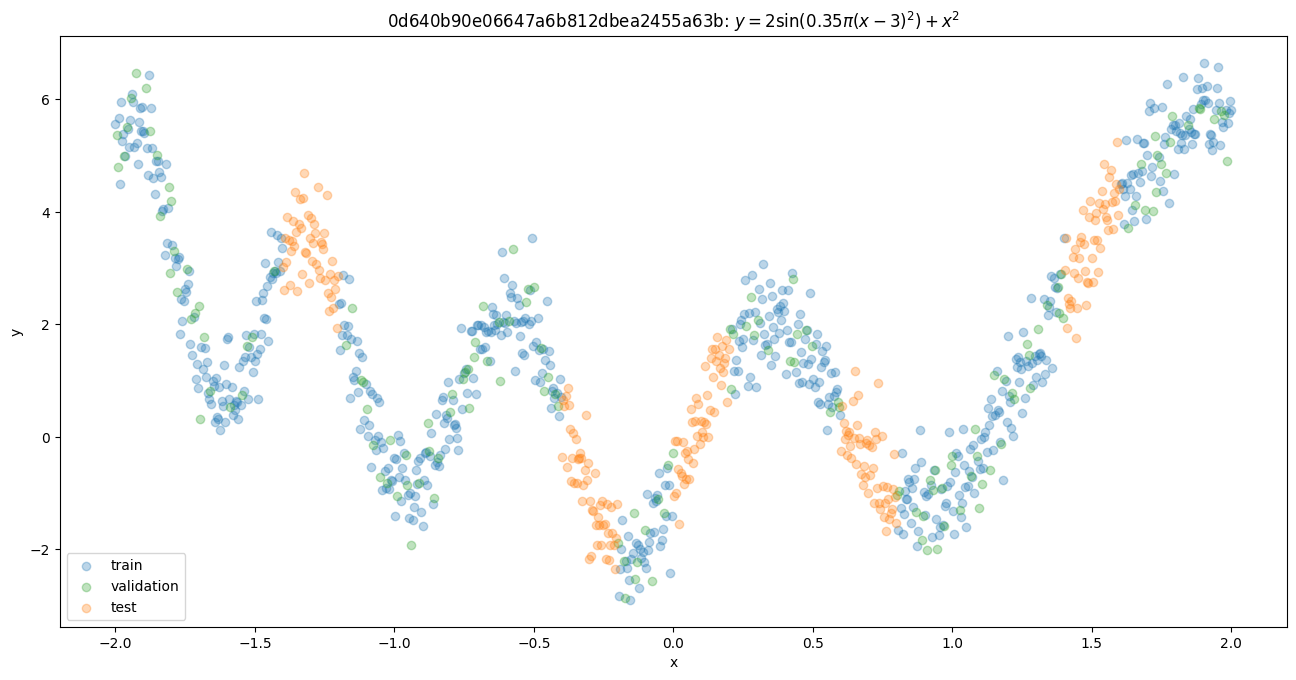
\includegraphics[width=\linewidth]{thesis-report/figures/toy_curves/data/curve0/data.png}
  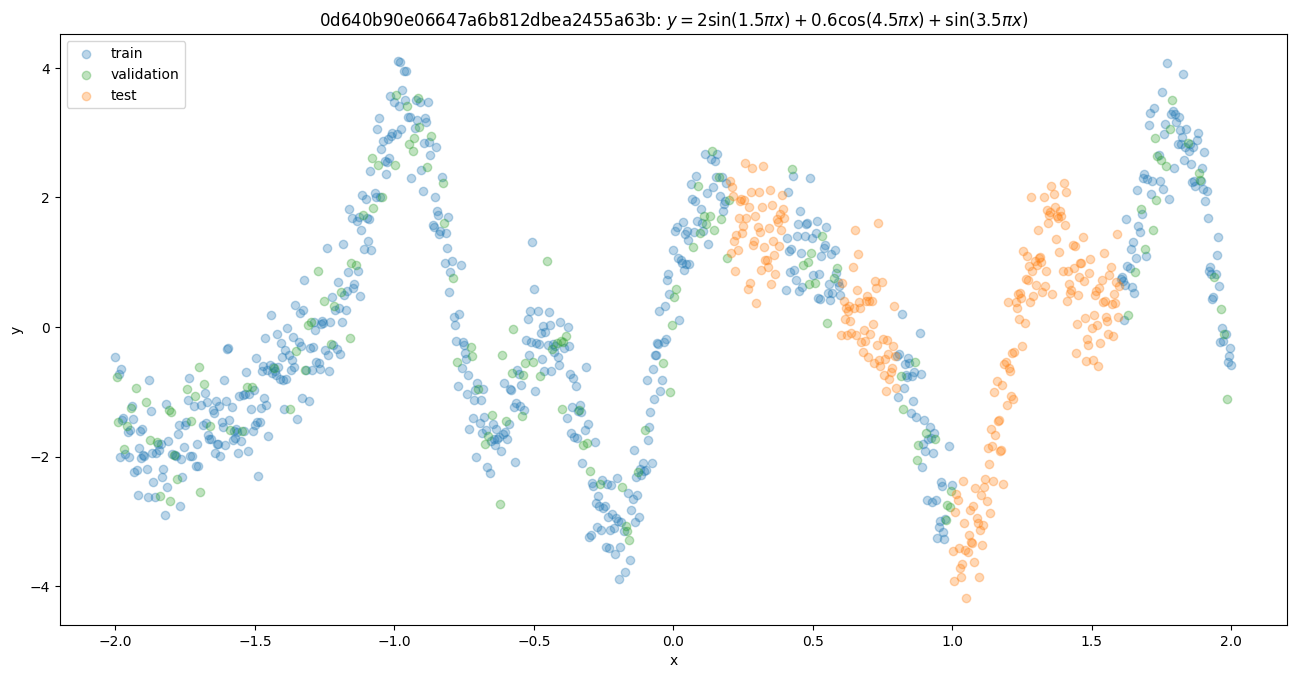
\includegraphics[width=\linewidth]{thesis-report/figures/toy_curves/data/curve3/data.png}
\end{minipage}%
\begin{minipage}{.49\textwidth}
  \centering
  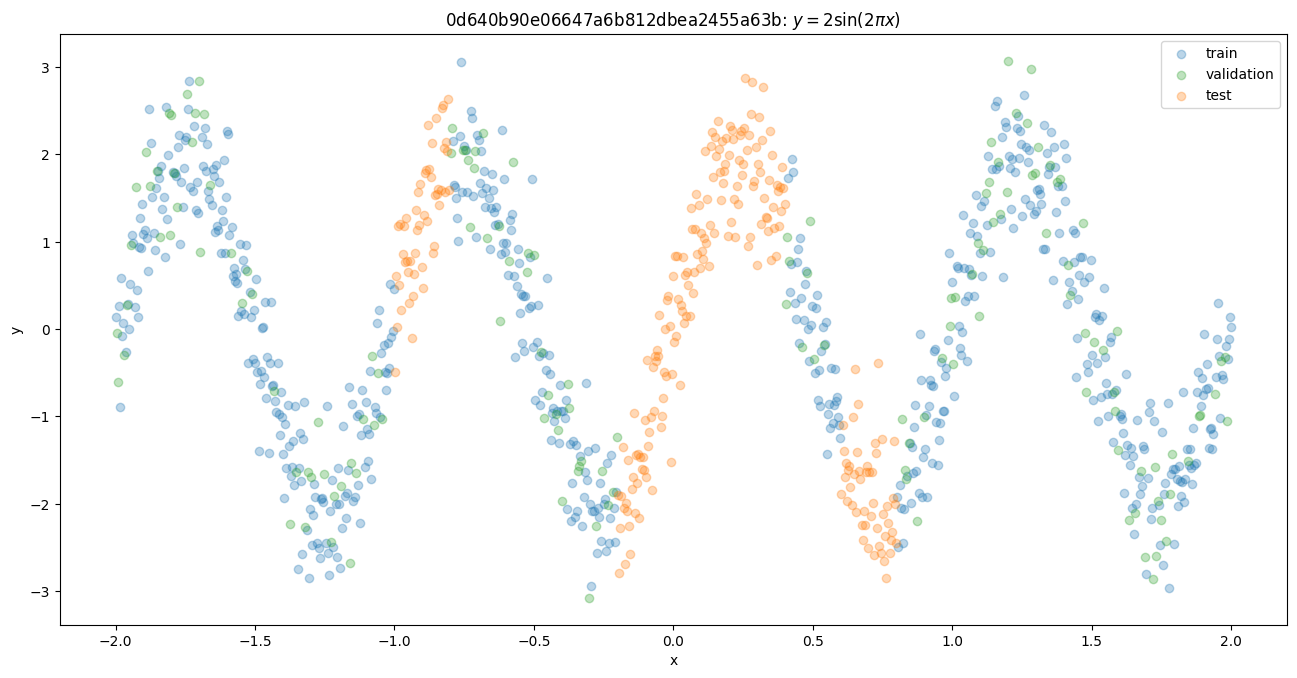
\includegraphics[width=\linewidth]{thesis-report/figures/toy_curves/data/curve1/data.png}
  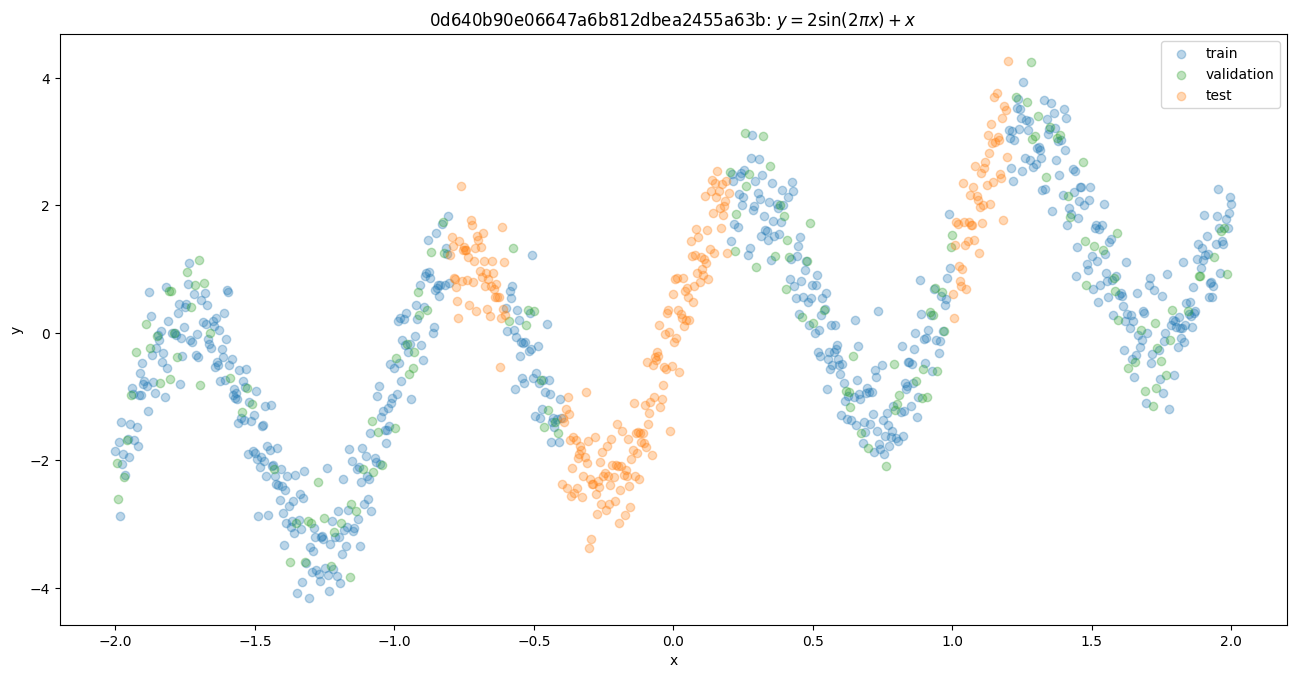
\includegraphics[width=\linewidth]{thesis-report/figures/toy_curves/data/curve4/data.png}
\end{minipage}%
\label{inducing-points-and-kernel}
\caption{GPs learned with GWI or pGVI}
\end{figure}


The prior is an essential component of a Bayesian posterior belief update.
However in the context of GWI, the prior GP can be interpreted as a regulariser for empirical risk minimisation.
To prevent confusion in this discussion, we will call this the regulariser GP. In our experiments, we explore traditional regularisers constructed with the standard GP prior, having $\mathcal{O}(1)$ computational complexity. We also propose the GP regulariser
\begin{align}
    y \vert \mathbf{Z}, \mathbf{U}, \sigma^2
    \sim \mathcal{N}\left(\bar{m}(x), \bar{k}(x, x)\right),
    \label{gp-posterior-regulariser}
\end{align}
a `lightweight' Bayesian posterior formulated with the inducing points $\mathbf{Z}\in \mathcal{X}^M$ and corresponding responses $\mathbf{U} \in \mathbb{R}^M$.
This regulariser would violate the traditional interpretation of a prior as it would explicitly use training data twice during inference.
We loosen this interpretation with the optimisation-centric nature of GWI, viewing this regulariser as potentially better informed than the prior GP.
Our experiments show that this less traditional regulariser can sometimes construct a better learning objective for GWI-GPs.
Moreover, the computational tractability of GWI is maintained with inversions of $\mathbb{R}^{M\times M}$ matrices only, when evaluating (\ref{gp-posterior-regulariser}).
\jw{maybe some images visualising a prior GP regulariser, posterior GP regulariser, and the corresponding GWI-GPs learned from them}

The predictive posterior of GWI-GPs are tempered following \cite{wild2022generalized}. This involves learning a factor $\alpha_T < 0$ for the tempered kernel
\begin{align}
    r_T(\mathbf{X}, \mathbf{X}) = \alpha_T \left(r(\mathbf{X}, \mathbf{X})+\sigma^2 \mathbf{I}\right),
\end{align}
where $\alpha_T$ is learned through negative log-likelihood optimisation on $\GP(m_Q, r_T)$ for a hold-out validation set with the rest of the GP parameters held fixed. This will form the final tempered GWI-GP predictive posterior
\begin{align}
    y \sim \mathcal{N}(m_Q(x), \alpha_T \left( r(x, x)) + \sigma^2\right).
\end{align}
Tempering is also applied to classificaiton by constructing $\boldsymbol{\alpha} \coloneqq \left[\alpha_T^1 \dots \alpha_T^J\right]^T \in [0, \infty)^J$, a seperate tempering factor for each GP, and optimising the classification log-likelihood in (\ref{robust-max-function-expected-log-likelihood}).

\subsection{The Wasserstein Distance}
\cite{wild2022generalized} provides the batched approximation of the Wasserstein distance from (\ref{wasserstein-distance}) for $N$ data points as
\begin{align}
    \mathbb{W}\left[Q, P\right]^2  &\approx \frac{1}{N_B}\sum_{n_b=1}^{N_B} \left(m_P(x_{n_b}) - m_Q(x_{n_b})\right)^2 \nonumber \\
    & \qquad + \frac{1}{N_B} \sum_{n_b=1}^{N_B} k(x_{n_b}, x_{n_b}) + \frac{1}{N_B} \sum_{n_b=1}^{N_B} r(x_{n_b}, x_{n_b}) \nonumber \\
    & \qquad - \frac{2}{\sqrt{N_B N_S}} \sum_{n_s=1}^{N_S} \sqrt{\lambda_{n_s}\left\big(r\left(\mathbf{X}_{N_S}, \mathbf{X}_{N_B}\right)k\left(\mathbf{X}_{N_B}, \mathbf{X}_{N_S}\right)\right\big)},
    \label{wasserstein-distance-approximation}
\end{align}
where $N_B < N$ and $N_S < N$ are two independent batches from the full data and $\lambda_{n}(\cdot)$ evaluates the $n^{th}$ eigenvalue.


In our experiments, we use the same data sample for $\mathbf{X}_{N_B}$ and $\mathbf{X}_{N_S}$, to ensure symmetric square matrices for $r\left(\mathbf{X}_{N_S}, \mathbf{X}_{N_B}\right)$ and $k\left(\mathbf{X}_{N_B}, \mathbf{X}_{N_S}\right)$ in the eigen-decomposition term of (\ref{wasserstein-distance-approximation}). This allows us to take advantage of eigenvalue properties of symmetric matrices, further explained in Appendix \ref{appendix:eigenvalue-symmetric-matrix}. We use symmetric matrices to leverage the eigendecomposition implementation in version 0.4 of Python JAX which is only available on GPUs for symmetric matrices. Our experiments show that using the same batch for $\mathbf{X}_{N_S}$ and $\mathbf{X}_{N_B}$ don't seem to make any significant difference on the resulting GWI-GP.
\jw{Include plots comparing GWI-GPs learned with the symmetric and non-symmetric}

The eigendecomposition in the last term of (\ref{wasserstein-distance-approximation}) is computationally expensive with $\mathcal{O}(N^3)$ complexity, which in our case is the sample size $N_S$.
In our experiments we found that we can often drop this last term during GWI with minor effect on the learned GWI-GP.
This trade-off of having a slightly imprecise Wasserstein distance significantly improves the speed of gradient computations during GWI.
\jw{Include plots comparing GWI-GPs learned with the full Wasserstein distance vs partial Wasserstein distance}

\newpage
\section{Projected Generalised Variational Inference for Gaussian Processes}
This section proposes a new learning framework called projected GVI (pGVI) for GPs to learn variational GPs we call pGVI-GPs.
pGVI uses the same GWI procedure in Algorithm \ref{alg:gwi-gp}, except it replaces the Wasserstein regularisation with a new form of regularisation we call projected regularisation.
Projected regularisations are significantly cheaper computationally, making pGVI an extremely attractive option in practice.
This section presents projected regularisations, followed by some visualisations of pGVI-GPs as qualitative motivation for the potential of this approach.

\subsection{Projected Regularisation}
The GVI framework from \cite{knoblauch2022optimization} assumes
\begin{align}
    \mathbb{D}\left[Q, P\right] = 0 \Leftrightarrow P = Q,
\end{align}
in other words, that the regulariser $\mathbb{D}$ is definite.
We propose dropping this assumption and choosing regularisers of the form
\begin{align}
    \mathbb{D}\left[Q, P\right] = \sum_{{n}=1}^{N} \mathbb{D}_0 \Big[\mathbb{Q}\left(F(x_n)\right), \mathbb{P}\left(F(x_n)\right)\Big],
    \label{projected-regulariser}
\end{align}
where $\mathbb{D}_0$ is a (base) regulariser between two probability measures on $\mathbb{R}$ and $x_n \in \mathcal{X}$.
Specifically, since both the variational and prior are GPs, we have that $\mathbb{Q}\left(F(x_n)\right) = \mathcal{N}\left(m_Q(x_n), r(x_n, x_n)\right)$ and $\mathbb{P}\left(F(x_n)\right) = \mathcal{N}\left(m_P(x_n), k(x_n, x_n)\right)$.
Therefore any base regulariser $\mathbb{D}_0$ that can be computed between two Gaussian random variables will lead to a tractable regulariser computation and therefore a tractable variational loss. We call regularisation schemes following (\ref{projected-regulariser}), projected regularisation.

We acknowledge that by only regularising against the marginal function values, we will be unconstrained with respect to correlations.
However our experiments suggest that this can act as a  sufficient regulariser to reap most of the benefits of GVI in terms of uncertainty quantification, while having significantly cheaper computational costs than GWI-GP learning or any other previous approach to function space VI such as \jw{[CITATIONS]}.

Projected regularisations are very cheap to compute.
The base regularisers that we propose are between scalar random variables having $\mathcal{O}(1)$ computational complexity for each training input $x_n$.
With $N$ points, we have $\mathcal{O}(N)$ complexity, significantly cheaper than the Wasserstein distance in (\ref{wasserstein-distance-approximation}), which is $\mathcal{O}(N^3)$. 

We will now review the base regularisers $\mathbb{D}_0$ used in our experiments. The Bhattacharyya distance is
\begin{align}
    \mathbb{B} \left[Q_{x}, P_{x}\right] &= \frac{1}{4} \frac{\left(\mu_p - \mu_q\right)^2}{\sigma_p^2 + \sigma_q^2} + \frac{1}{2} \log\left(\frac{\sigma_p^2 + \sigma_q^2}{2\sigma_p\sigma_q^}\right),
\end{align}
where $Q_{x} \coloneqq \mathbb{Q}\left(F(x)\right)$, $P_{x} \coloneqq \mathbb{P}\left(F(x)\right)$, $\mu_p \coloneqq m_P(x)$, $\mu_q \coloneqq m_Q(x)$, $\sigma_p^2 \coloneqq k(x, x)$, and $\sigma_q^2 \coloneqq r(x, x)$.
The squared 2-Wasserstein distance for Gaussians on $\mathbb{R}$ is
\begin{align}
    \mathbb{W} \left[Q_{x}, P_{x}\right]^2 &= \left(\mu_p - \mu_q\right)^2 + \sigma_p^2 + \sigma_q^2 - 2 \sigma_p\sigma_q.
\end{align}
The Hellinger distance is
\begin{align}
    \mathbb{H} \left[Q_{x}, P_{x}\right] = 1 - \sqrt{\frac{2\sigma_p\sigma_q}{\sigma_p^2 + \sigma_q^2}} \exp\left(\frac{1}{4} \frac{ \left(\mu_p - \mu_q\right)^2}{\sigma_p^2 + \sigma_q^2}\right).
\end{align}
The KL divergence for measures on $\mathbb{R}$ is
\begin{align}
    \mathbb{KL} \left[Q_{x}, P_{x}\right] &= \log\frac{\sigma_q^2}{\sigma_p^2} + \frac{\sigma_p^2 + \left(\mu_p - \mu_q\right)^2}{2 \sigma_q^2} - \frac{1}{2}.
\end{align}
The $\alpha$-Renyi divergence is
\begin{align}
    \mathbb{R}_\alpha \left[Q_{x}, P_{x}\right] &= \log\frac{\sigma_p}{\sigma_q} + \frac{1}{2(\alpha-1)}\log\left(\frac{\sigma_p^2}{\alpha \sigma_p^2 + (1-\alpha) \sigma_q^2}\right)  + \frac{1}{2}\frac{\alpha \left(\mu_p - \mu_q\right)^2}{\alpha \sigma_p^2 + (1-\alpha) \sigma_q^2},
\end{align}
with $\alpha \sigma_p^2 + (1-\alpha) \sigma_q^2 > 0$.
Finally, we also experimented with a naive divergence
\begin{align}
    \mathbb{N} \left[Q_{x}, P_{x}\right] = \left(\mu_p - \mu_q\right)^2 + \left(\sigma_q^2-\sigma_p^2\right)^2,
\end{align}
taking the squared difference of the means and covariances.

\subsection{Regression Visualisations}
\jw{Some visualistions of pGVI-GPs}

\newpage
\section{Experimentation Framework}
This section presents the experimentation framework that we developed for learning GWI-GPs and pGVI-GPs.
We begin by describing our implementation architecture followed by our setup for scaling experimentation.
Finally we will present results for some 1-D curve regression problems to show our framework in action.
Our most up-to-date\footnote{We include the most up-to-date version of the implementation for future reference. For grading purposes, please refer to \href{https://github.com/jswu18/generalised-variational-inference-for-gaussian-processes/tree/7b81dd607ef2ace4b66f9440becb2722be0eb9e6}{this commit} as the last version prior to the submission date: \href{https://github.com/jswu18/generalised-variational-inference-for-gaussian-processes/tree/7b81dd607ef2ace4b66f9440becb2722be0eb9e6}{https://github.com/jswu18/generalised-variational-inference-for-gaussian-processes/tree/7b81dd607ef2ace4b66f9440becb2722be0eb9e6}} Python implementation is openly available on \href{https://github.com/jswu18/generalised-variational-inference-for-gaussian-processes}{GitHub}\footnote{\href{https://github.com/jswu18/generalised-variational-inference-for-gaussian-processes}{https://github.com/jswu18/generalised-variational-inference-for-gaussian-processes}}.

\subsection{Implementation Architecture}\label{implementation-architecture}
GWI and pGVI are highly flexible learning frameworks. As such, abstraction was critical to ensuring a scaleable and maintainable implementation architecture.
Luckily, the GVI framework proposed by \cite{knoblauch2022optimization} naturally translates to a clear implementation architecture that we have developed and visualised in Figure \ref{gvi-implementation}.
We see that the GVI objective in (\ref{gvi-posterior-in-fs}) with $\ell$ and $\mathbb{D}$ has been abstracted to accommodate any valid empirical risk and regularisation, respectively.
These abstractions are exactly mirrored in our implementation architecture as abstract base classes ensuring the same interface is inherited by all child class implementations.
\begin{figure}[h!]
\begin{center}
\resizebox{\textwidth}{!}{
\begin{tikzpicture}

\begin{class}[text width=5cm]{GVI}{0,0}
\attribute{empirical risk : EmpiricalRisk}
\attribute{regularisation : Regularisation}
\operation{calculate ( $\gamma$ , $\mathbf{X}$ , $\mathbf{Y}$ ) : Float}
\end{class}

\begin{abstractclass}[text width=5cm]{EmpiricalRisk}{-6,-3}
\attribute{$Q$ : ApproximateGP}
\operation{calculate ( $\gamma$ , $\mathbf{X}$ , $\mathbf{Y}$ ) : Float}
\end{abstractclass}


\begin{class}[text width=5cm]{NegativeLogLikelihood}{-9,-6}
\inherit{EmpiricalRisk}
\end{class}

\begin{class}[text width=5cm]{CrossEntropy}{-3,-6}
\inherit{EmpiricalRisk}
\end{class}

\begin{abstractclass}[text width=5cm]{Regularisation}{6 , -3}
\attribute{$P$ : ExactGP}
\attribute{$\theta$ : ExactGP Parameters}
\attribute{$Q$ : ApproximateGP}
\attribute{mode : \{`prior', `posterior'\}}
\operation{calculate ( $\gamma$ , $\mathbf{X}$ ) : Float}
\end{abstractclass}

\begin{class}[text width=5cm]{Wasserstein}{9,-7.5}
\inherit{Regularisation}
\attribute{include eigendecomp. : Bool}
\end{class}

\begin{abstractclass}[text width=5cm]{ProjectedRegularisation}{0,-7.5}
\inherit{Regularisation}
\attribute{$D$ : Int}
\end{abstractclass}

\begin{class}[text width=5cm]{Bhattacharyya}{-9,-9.25}
\inherit{ProjectedRegularisation}
\end{class}

\begin{class}[text width=5cm]{Wasserstein}{-9,-11}
\inherit{ProjectedRegularisation}
\end{class}

\begin{class}[text width=5cm]{Hellinger}{-3,-11}
\inherit{ProjectedRegularisation}
\end{class}

\begin{class}[text width=5cm]{KL}{3,-11}
\inherit{ProjectedRegularisation}
\end{class}

\begin{class}[text width=5cm]{Renyi}{9,-11}
\inherit{ProjectedRegularisation}
\attribute{$\alpha$ : Float}
\end{class}

\begin{class}[text width=5cm]{SquaredDifference}{9,-9.25}
\inherit{ProjectedRegularisation}
\end{class}

\composition{GVI}{}{}{EmpiricalRisk}
\composition{GVI}{}{}{Regularisation}

\end{tikzpicture}
}
\caption{GVI Implementation Architecture}
\label{gvi-implementation}
\end{center}
\end{figure}

Algorithms \ref{alg:inducing-point-selection}, \ref{alg:gwi-gp}, and \ref{alg:inducing-points-prior-gp} are also in an abstracted form, accomodating any valid mean $m_P$ or $m_Q$, kernel $k$, and variational kernel $r$. We developed the architecture in Figure \ref{gp-implementation} for our implementation of GPs, Figure \ref{mean-implementation} for mean functions, and Figure \ref{kernel-implementation} for kernels. These architectures are clearly reflected in our code base.
\begin{figure}[h!]
\begin{center}
\resizebox{\textwidth}{!}{
\begin{tikzpicture}

\begin{abstractclass}[text width=5cm]{GP}{0, 4}
\attribute{$m$ : Mean}
\attribute{$k$ : Kernel}
\end{abstractclass}

\begin{abstractclass}[text width=5cm]{ExactGP}{-9, 1.25}
\inherit{GP}
\operation{predict ( $\theta$ , $\mathbf{X}$ ) : Distribution}
\end{abstractclass}

\begin{abstractclass}[text width=5cm]{ApproxGP}{-3, 1.25}
\inherit{GP}
\operation{predict ( $\gamma$ , $\mathbf{X}$ ) : Distribution}
\end{abstractclass}

\begin{abstractclass}[text width=5cm]{GPClassification}{3, 1.25}
\inherit{GP}
\attribute{dist. : Dist = Multinomial}
\end{abstractclass}

\begin{abstractclass}[text width=5cm]{GPRegression}{9, 1.25}
\inherit{GP}
\attribute{dist. : Dist. = Gaussian}
\end{abstractclass}

\begin{class}[text width=5cm]{ExactGPRegression}{-9, -2.5}
\inherit{ExactGP}
\inherit{GPRegression}
\end{class}

\begin{class}[text width=5cm]{ApproxGPRegression}{-3, -2.5}
\inherit{ApproxGP}
\inherit{GPRegression}
\end{class}

\begin{class}[text width=5cm]{ExactGPClassification}{3, -2.5}
\inherit{ExactGP}
\inherit{GPClassification}
\end{class}

\begin{class}[text width=5cm]{ApproxGPClassification}{9, -2.5}
\inherit{ApproxGP}
\inherit{GPClassification}
\end{class}

\begin{abstractclass}[text width=5cm]{Mean}{-9, 3.85}
\operation{predict ( $\theta_{m}$ , $\mathbf{X}$ ) : Array}
\end{abstractclass}

\begin{abstractclass}[text width=5cm]{Kernel}{9, 3.85}
\operation{gram ( $\theta_{k}$ , $\mathbf{X}$ ) : Array}
\end{abstractclass}

\composition{GP}{}{}{Mean}
\composition{GP}{}{}{Kernel}
\end{tikzpicture}
}
\caption{GP Implementation Architecture}
\label{gp-implementation}
\end{center}
\end{figure}


\begin{figure}[h!]
\begin{center}
\resizebox{0.75\textwidth}{!}{
\begin{tikzpicture}
\begin{abstractclass}[text width=5cm]{Mean}{0, 0}
\operation{predict ( $\theta_{m}$ , $\mathbf{X}$ ) : Array}
\end{abstractclass}

\begin{class}[text width=5cm]{Constant}{0, -3}
\inherit{Mean}

\end{class}
\begin{class}[text width=5cm]{SVGP}{-6, -3}
\attribute{$m_P$ : Mean}
\attribute{$\theta_{m_P}$ : Mean Parameters}
\attribute{$k$ : Kernel}
\attribute{$\theta_{k}$ : Kernel Parameters}
\attribute{$\mathbf{Z}$ : Array}
\inherit{Mean}
\end{class}

\begin{class}[text width=5cm]{NeuralNetwork}{6, -3}
\attribute{architecture : List}

\inherit{Mean}
\end{class}
\end{tikzpicture}
}
\caption{Mean Implementation Architecture}
\label{mean-implementation}
\end{center}
\end{figure}



\begin{figure}[h!]
\begin{center}
\resizebox{\textwidth}{!}{
\begin{tikzpicture}
\begin{abstractclass}[text width=5cm]{Kernel}{4, 0}
\operation{gram ( $\theta_{k}$ , $\mathbf{X}$ ) : Array}
\end{abstractclass}

\begin{class}[text width=5cm]{Polynomial}{-2, -1.5}
\attribute{degree : Float}
\inherit{Kernel}
\end{class}

\begin{class}[text width=5cm]{SquaredExponential}{-2, -4}
\inherit{Kernel}
\end{class}

\begin{class}[text width=5cm]{NeuralNetwork}{10, -4}
\attribute{$k_0$ : Kernel}
\attribute{$h$ : NeuralNetwork}
\inherit{Kernel}
\end{class}

\begin{class}[text width=5cm]{NNGP}{10, -1.5}
\attribute{architecture: List}
\inherit{Kernel}
\end{class}



\begin{abstractclass}[text width=5cm]{Approximate}{4, -4}
\inherit{Kernel}
\attribute{$\mathbf{Z}$ : Array}
\end{abstractclass}

\begin{abstractclass}[text width=5cm]{SVGP}{1, -7}
\inherit{Approximate}
\attribute{$k$ : Kernel}
\attribute{$\theta_{k}$ : Kernel Parameters}
\end{abstractclass}

\begin{class}[text width=5cm]{SparsePosterior}{7, -7}
\inherit{Approximate}
\attribute{$r_0$ : Kernel}
\end{class}

\begin{class}[text width=5cm]{FixedSparsePosterior}{13, -7}
\inherit{Approximate}
\attribute{$k$ : Kernel}
\attribute{$\theta_{k}$ : Kernel Parameters}
\attribute{$r_0$ : Kernel}
\end{class}

\begin{class}[text width=5cm]{CholeskySVGP}{-5, -10.5}
\inherit{SVGP}
\end{class}

\begin{class}[text width=5cm]{DiagonalSVGP}{1, -10.5}
\inherit{SVGP}
\end{class}

\begin{class}[text width=5cm]{KernelisedSVGP}{7, -10.5}
\attribute{$r_0$ : Kernel}
\inherit{SVGP}
\end{class}

\end{tikzpicture}
}
\caption{Kernel Implementation Architecture}
\label{kernel-implementation}
\end{center}
\end{figure}

Our implementation is in Python and predominantly uses JAX, a high-performance numerical computing package developed by \cite{jax2018github}.
Because there is currently no stable, well-maintained, and well-documented implementation of GPs with JAX, all implementations were essentially developed from scratch for the purposes of this project.
We chose JAX for its currently growing user-base, unique customisations, and to ensure compatibility with the implementation of NNGP kernels by \cite{novak2019neural}, which is also developed in JAX.
We chose Python for its current popularity within the machine learning community.
To ensure numerical stability, we incorporated a number of commonly used implementation techniques such as adding jitter and using the Cholesky decomposition for matrix inversions, when necessary.

As we continue to grow the code base, we incorporated a number of standard software engineering tools to ensure a scaleable, maintainable, and controlled implementation environment.
We introduce strict typing controls for all model parameter classes with Pydantic base models from \cite{samuel_colvin_2023_8277473}.
Pydantic models enforce typing hints during run-time that would otherwise be considered `syntactic sugar' in Python. This also provides clear guidelines when constructing GPs within our framework.
Our implementation also includes a rigorous testing environment that currently has 95\% test coverage over the implementations found in the \code{src/} directory, much higher than needed in most software development projects.
This also includes mockers for isolated testing of different components (i.e. mockers for means and kernels to isolate testing of GP implementations). Finally, we use Poetry developed by \cite{Eustace} to strictly control package requirements, ensuring the version compatibility of dependencies.

\subsection{Scaling Experiments}
In addition to our implementation architecture, we developed a scaleable solution for performing large numbers of experiments.
Implemented in the \code{experiments/} directory, we constructed schemas and resolvers for each abstraction in Section \ref{implementation-architecture}.
This allows us to define and construct experiments through \code{.yaml} configuration files.
Each \code{.yaml} outlines the configuration settings required to define an experiment i.e. the GP, learning objective, learning rate, optimiser, etc. Appendix \ref{appendix:regulariser-yaml} and \ref{appendix:approximate-yaml} show example \code{.yaml} configuration files used for learning a regulariser GP and approximate GP respectively.

Generating configuration files was automated to scale our experiments to try all possible combinations of empirical risks, regularisers, mean functions, and kernels. These configurations were then submitted as jobs to a computing cluster, running our experiments in a organised and scaleable framework.

\subsection{Regression Curve Experiments}
To demonstrate our experimentation framework, we learned GWI-GPs and pGVI-GPs for ten regression curves. 
Each curve has randomly selected segments removed from the training data to visualise an out-of-data (OOD) setting.
With our framework, we constructed 1513 experiments for each curve, each defined through \code{.yaml} configuration files. 
Each experiment is a unique construction of a regulariser GP, an approximate GP, and a GVI objective (among other settings). 
After performing all experiments, we select the configuration with the best performance. 
Given the setup of these regression curve problems, we selected based on the highest negative-log-likelihood with respect to the training data. 
In other problem regimes, it maybe more suitable to select based on test set performance. 
We visualise four GPs in Figure \ref{toy-curves-gps}, the best performing GWI-GP or pGVI-GPs for their respective curve problem. 
The rest of the curves are visualised in Appendix \ref{appendix:toy-curves}.

\begin{figure}[h!]
\centering
\begin{minipage}{.49\textwidth}
  \centering
  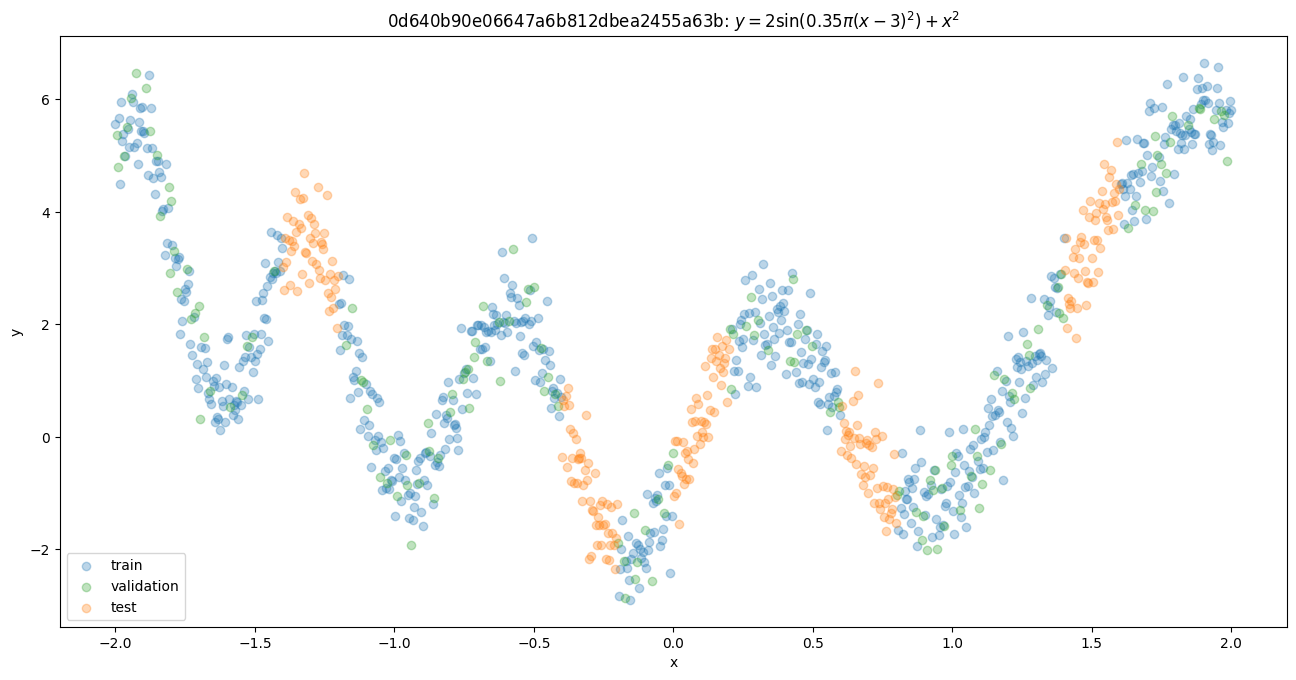
\includegraphics[width=\linewidth]{thesis-report/figures/toy_curves/data/curve0/data.png}
  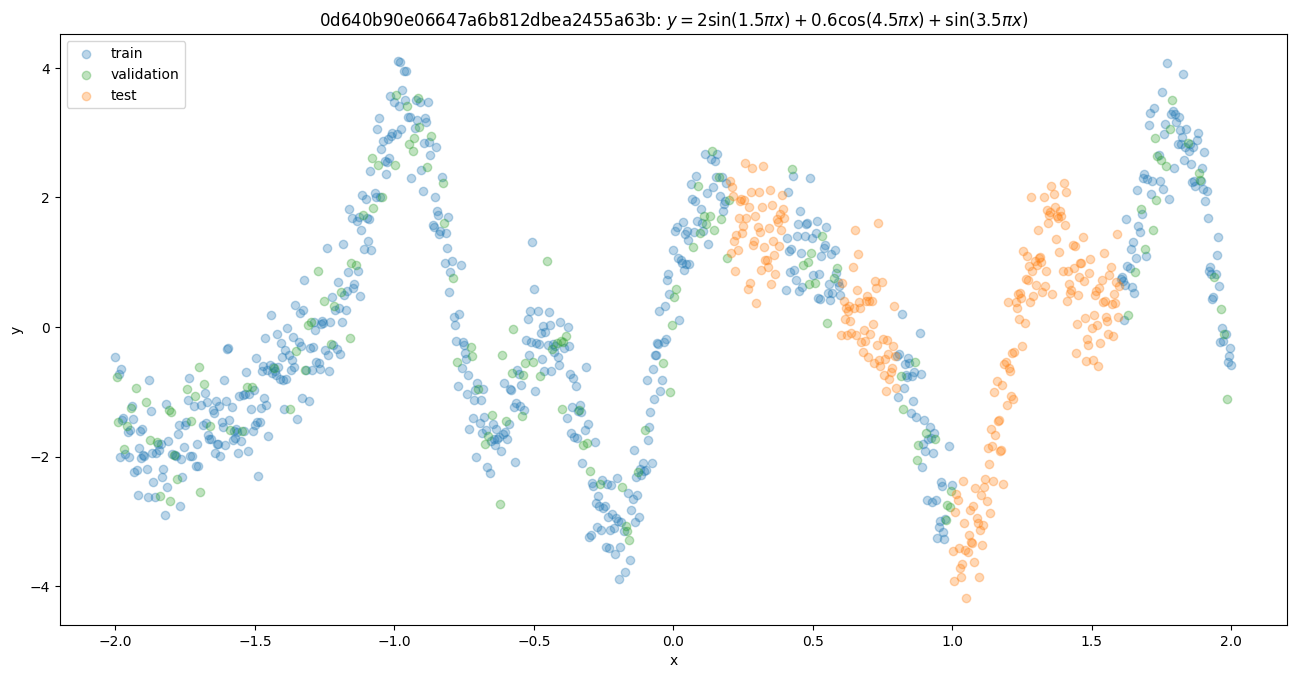
\includegraphics[width=\linewidth]{thesis-report/figures/toy_curves/data/curve3/data.png}
\end{minipage}%
\begin{minipage}{.49\textwidth}
  \centering
  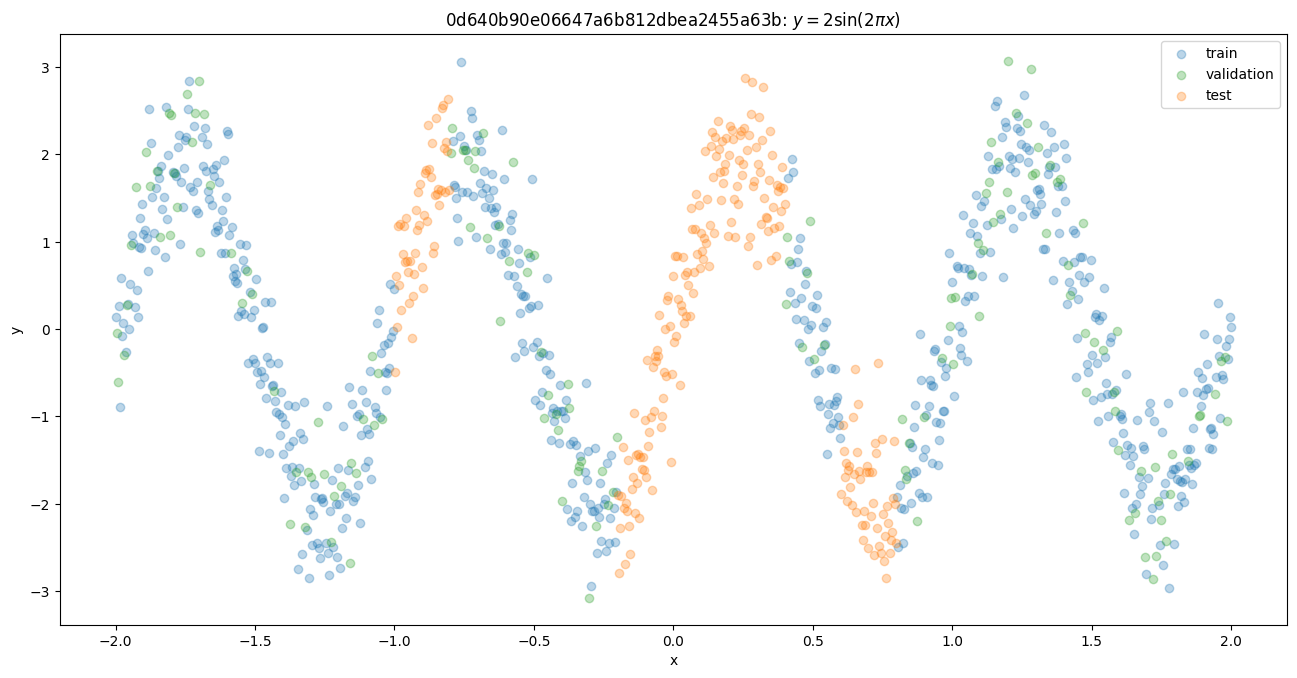
\includegraphics[width=\linewidth]{thesis-report/figures/toy_curves/data/curve1/data.png}
  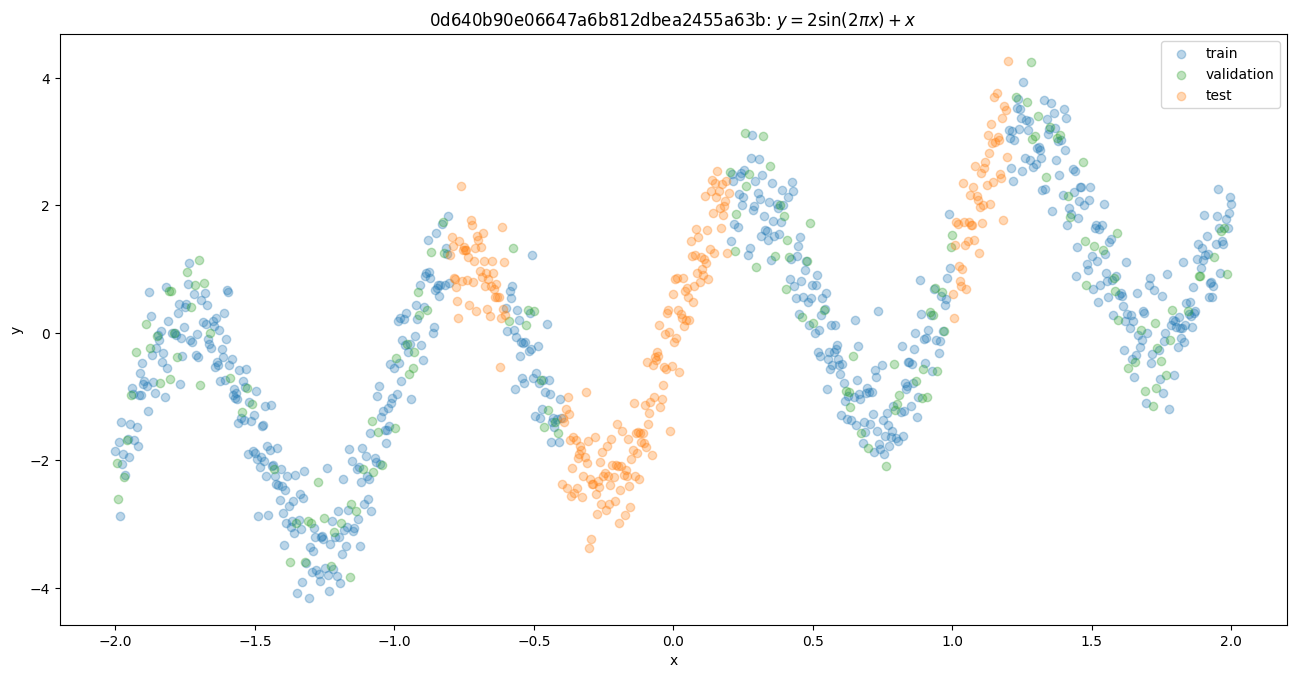
\includegraphics[width=\linewidth]{thesis-report/figures/toy_curves/data/curve4/data.png}
\end{minipage}%
\label{toy-curves-gps}
\caption{GPs learned with GWI or pGVI}
\end{figure}

Additionally, Table X presents a subset of the configurations resulting in each of these best performing variational GPs. 
This table gives an idea of the large space of settings available within GWI and pGVI. 
It also demonstrates the flexibility of the learning frameworks to accommodate different approximate spaces and learning objectives that may be better suited for a specific problem. 

\newpage
\section{Future Work}

\subsection{Inducing Points Selection}
\jw{Not using actual data points}
\jw{Not selecting actual training points, but learning points that are most representative of the data? i.e. naively a convex combination of images, or weight params in a single layer NN.}
\jw{Selecting in a Feature Space}
\jw{i.e. choosing inducing points from the feature representation of the data points from a NN feature extractor}


\subsection{Applications to Different Problem Domains}

\jw{Regression}

\jw{Image Classification}


\jw{NLP Named-Entity Recognition}
\jw{Putting pre-trained transformers in the mean and kernels.}



\newpage
\section{Conclusions}


\newpage
\bibliography{references}


\newpage
\appendix
\section{Appendix}
\subsection{Positive Semi-Definite Kernels} \label{appendix:positive-definite-kernel}
For a kernel function $k: \mathcal{X} \times \mathcal{X} \rightarrow \mathbb{R}$ defined as an inner product of features in some feature space $\mathcal{H}$:
\begin{align}
    k(x, x') = \langle \phi(x), \phi(x') \rangle_{\mathcal{H}}
\end{align}
where $\phi: \mathcal{X} \rightarrow \mathcal{H}$, a gram matrix $\mathbf{K} \in \mathbb{R}^{N\times N}$ defined element-wise:
\begin{align}
    \left[\mathbf{K}\right]_{n, n'} = k(x_n, x_{n'})
\end{align}
for any $N$ points $\mathbf{X} = \left\{x_n\right\}_{n=1}^N$ with $x_n \in \mathcal{X}$, and any vector $\mathbf{v} \in \mathbb{R}^N$ then:
\begin{align}
    \mathbf{v}^T \mathbf{K} \mathbf{v} &= \sum_{n=1}^N\sum_{n'=1}^N v_n v_{n'}  \left\langle \phi(x_n), \phi(x_{n'}) \right\rangle_{\mathcal{H}} \\
    &= \left\langle\sum_{n=1}^N v_n \phi(x_n), \sum_{n'=1}^N  v_{n'}\phi(x_{n'}) \right\rangle_{\mathcal{H}} \\
    &= \left\| \sum_{n=1}^N v_n \phi(x_n) \right\|^2 \geq 0
\end{align}
showing that $\mathbf{K}$ is a positive semi-definite matrix.

\newpage
\subsection{Symmetric Matrix Eigenvalues}\label{appendix:eigenvalue-symmetric-matrix}
For square symmetric matrices $\mathbf{A}, \mathbf{B} \in \mathbb{R}^{N \times N}$, $\sqrt{\mathbf{A}}\mathbf{B}\sqrt{\mathbf{A}}$ is also a symmetric matrix where $\sqrt{\mathbf{A}}$ is the square root such that $\mathbf{A} = \sqrt{\mathbf{A}}^T \sqrt{\mathbf{A}}$. Moreover,
\begin{align}
    \lambda_{n} \left(\mathbf{A} \mathbf{B}\right) = \lambda_{n} \left(\sqrt{\mathbf{A}}\mathbf{B}\sqrt{\mathbf{A}}\right)
\end{align}
where $\lambda_{n}(\cdot)$ computes the $n^{th}$ eigenvalue.

\newpage
\subsection{Example Regulariser GP YAML}\label{appendix:regulariser-yaml}
\begin{lstlisting}[style=yaml]
data_name: 604913dc3af2417fb1d5a21ea26e4afd
empirical_risk_break_condition: -10
empirical_risk_schema: negative_log_likelihood
inducing_points:
  inducing_points_factor: 1.0
  inducing_points_power: 3
  inducing_points_selector_schema: conditional_variance
kernel:
  kernel_kwargs:
    input_shape:
    - 1
    layers:
      layer_1:
        layer_kwargs:
          features: 10
        layer_schema: dense
      layer_2:
        layer_kwargs: null
        layer_schema: tanh
  kernel_parameters: null
  kernel_schema: nngp
number_of_iterations: 5
save_checkpoint_frequency: 1000
trainer_settings:
  batch_drop_last: false
  batch_shuffle: true
  batch_size: 1000
  learning_rate: 0.01
  number_of_epochs: 1000
  optimiser_schema: adam
  seed: 0
\end{lstlisting}

\newpage
\subsection{Example Approximate GP YAML}\label{appendix:approximate-yaml}

\begin{lstlisting}[style=yaml]
empirical_risk_schema: negative_log_likelihood
kernel:
  kernel_kwargs:
    diagonal_regularisation: 1.0e-10
    is_diagonal_regularisation_absolute_scale: false
  kernel_parameters: null
  kernel_schema: sparse_posterior
mean:
  mean_kwargs:
    nn_function_kwargs:
      input_shape:
      - 1
      layers:
        layer_1:
          layer_kwargs:
            features: 10
          layer_schema: dense
        layer_2:
          layer_kwargs: null
          layer_schema: tanh
        layer_3:
          layer_kwargs:
            features: 1
          layer_schema: dense
      seed: 0
    number_output_dimensions: 1
  mean_parameters: null
  mean_schema: custom
reference_name: 7b386a3faf1f4b79ac6ff6604b6bc932
regularisation:
  regularisation_kwargs:
    mode: posterior
  regularisation_schema: projected_renyi
save_checkpoint_frequency: 1000
trainer_settings:
  batch_drop_last: false
  batch_shuffle: true
  batch_size: 1000
  learning_rate: 0.01
  number_of_epochs: 1000
  optimiser_schema: adam
  seed: 0
\end{lstlisting}

\newpage
\subsection{Regression Curves}\label{appendix:toy-curves}
\begin{figure}[h!]
\centering
\begin{minipage}{.49\textwidth}
  \centering
  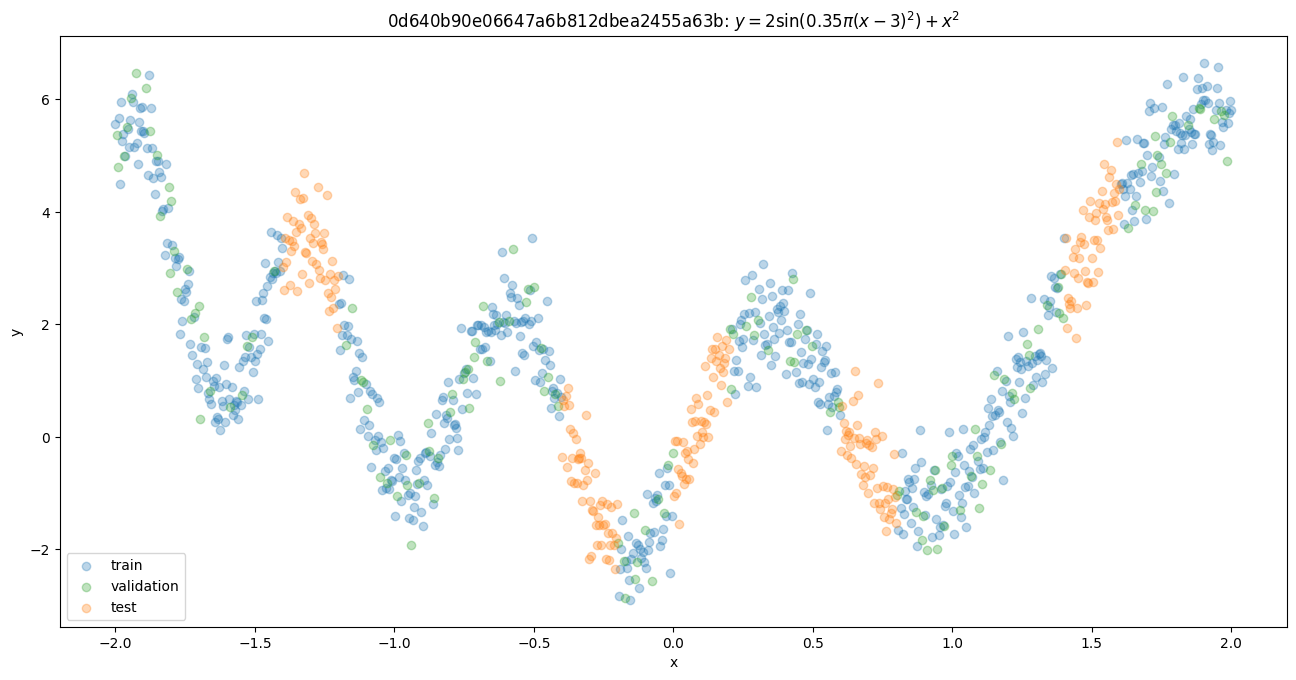
\includegraphics[width=\linewidth]{thesis-report/figures/toy_curves/data/curve0/data.png}
  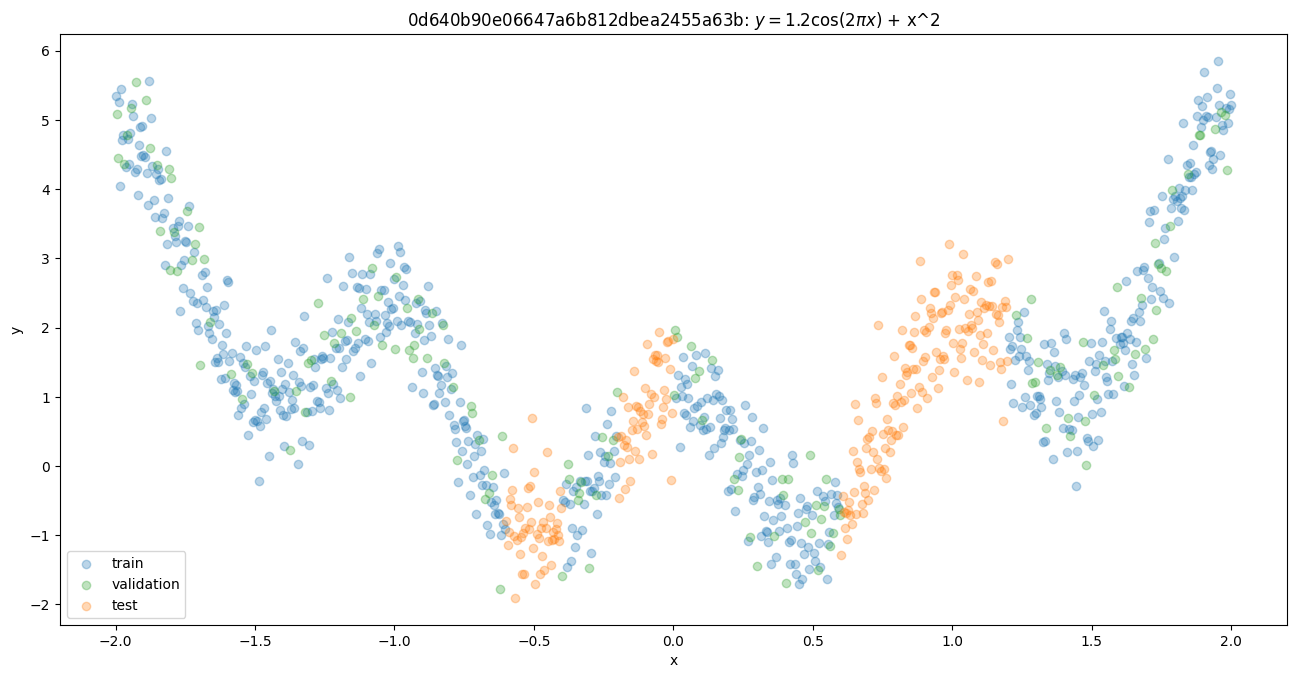
\includegraphics[width=\linewidth]{thesis-report/figures/toy_curves/data/curve2/data.png}
  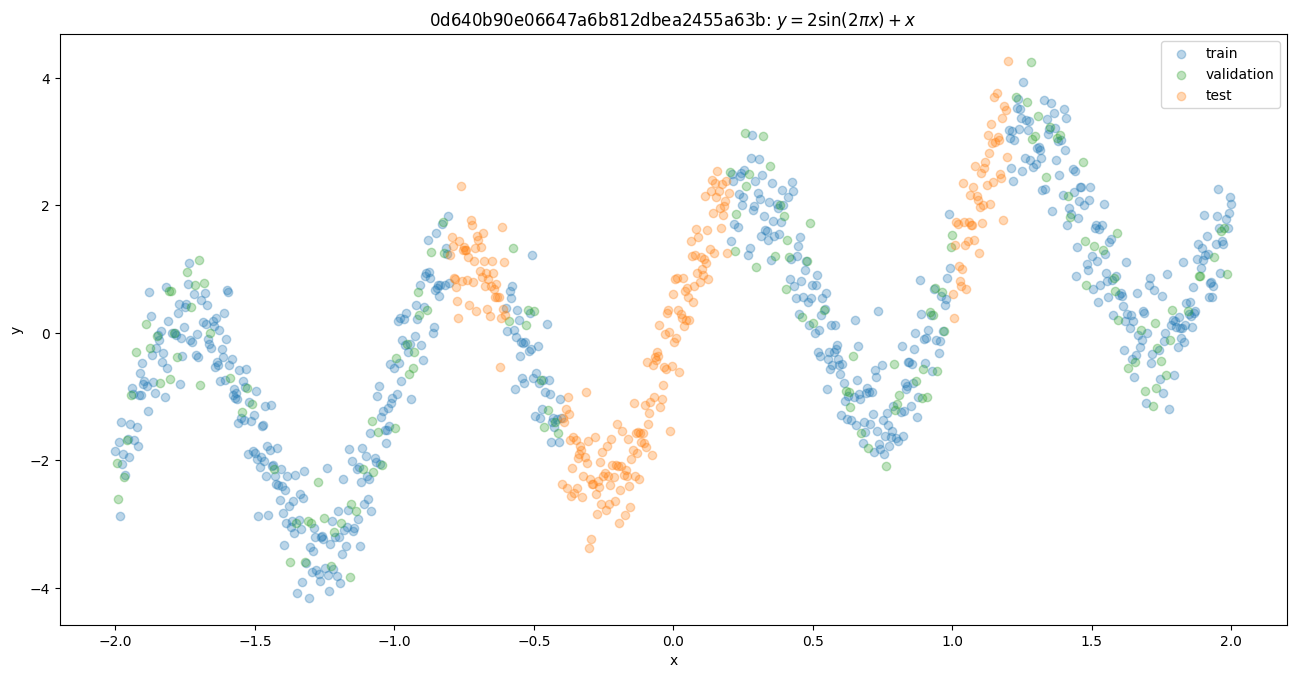
\includegraphics[width=\linewidth]{thesis-report/figures/toy_curves/data/curve4/data.png}
  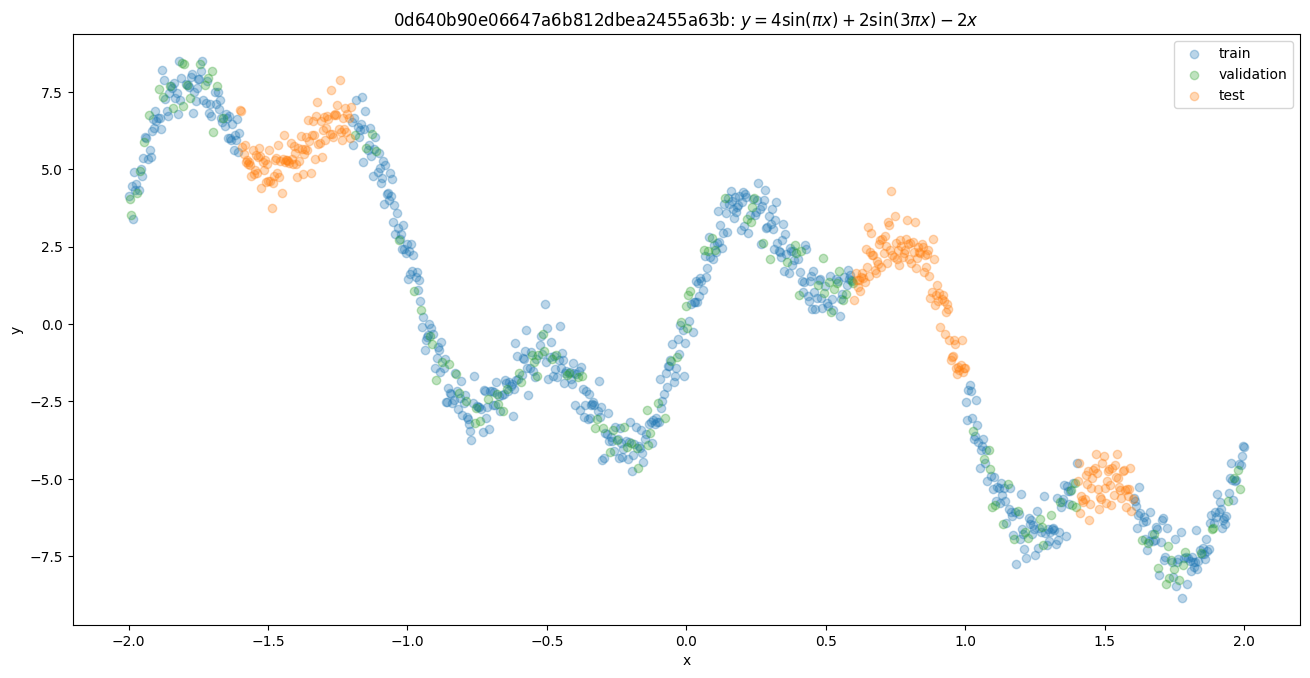
\includegraphics[width=\linewidth]{thesis-report/figures/toy_curves/data/curve6/data.png}
  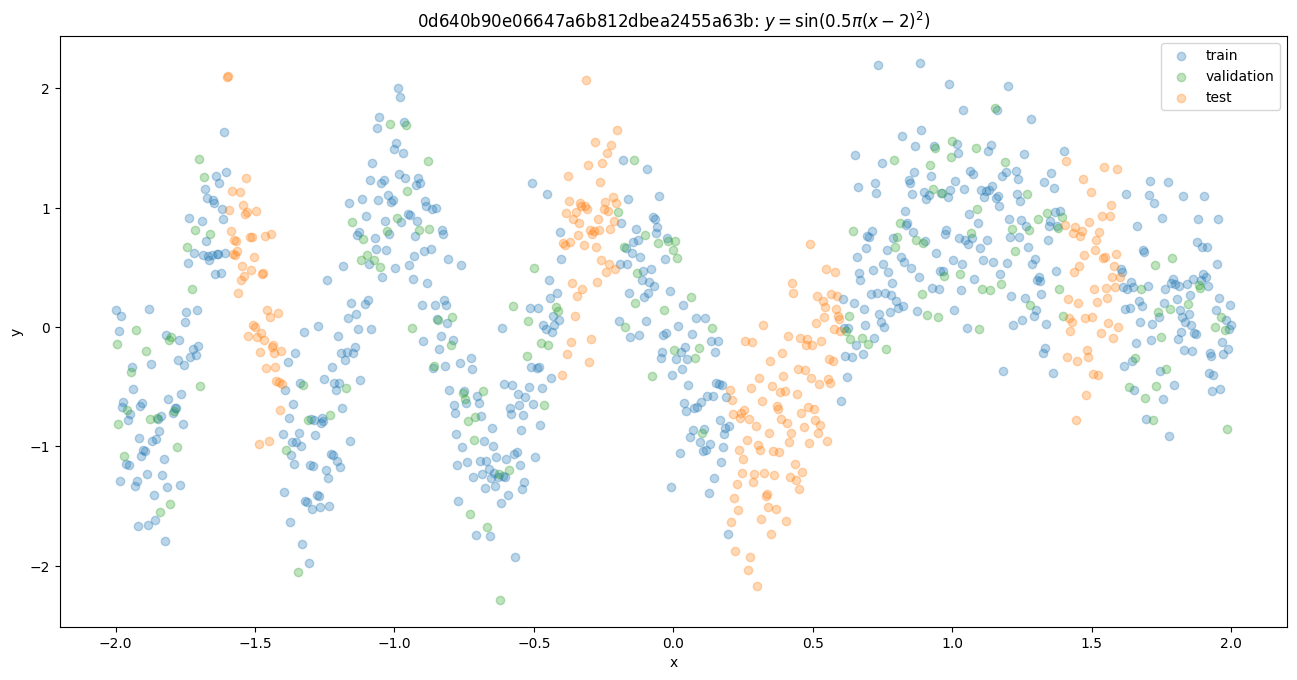
\includegraphics[width=\linewidth]{thesis-report/figures/toy_curves/data/curve8/data.png}
\end{minipage}%
\begin{minipage}{.49\textwidth}
  \centering
  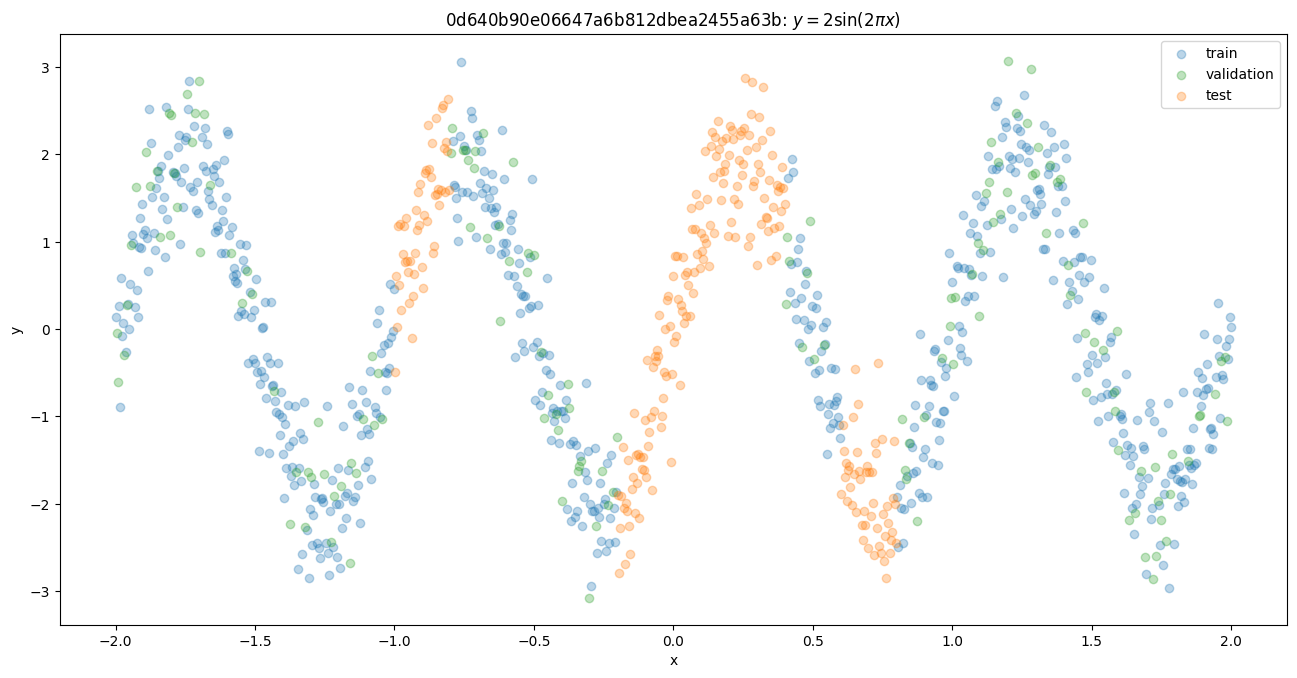
\includegraphics[width=\linewidth]{thesis-report/figures/toy_curves/data/curve1/data.png}
  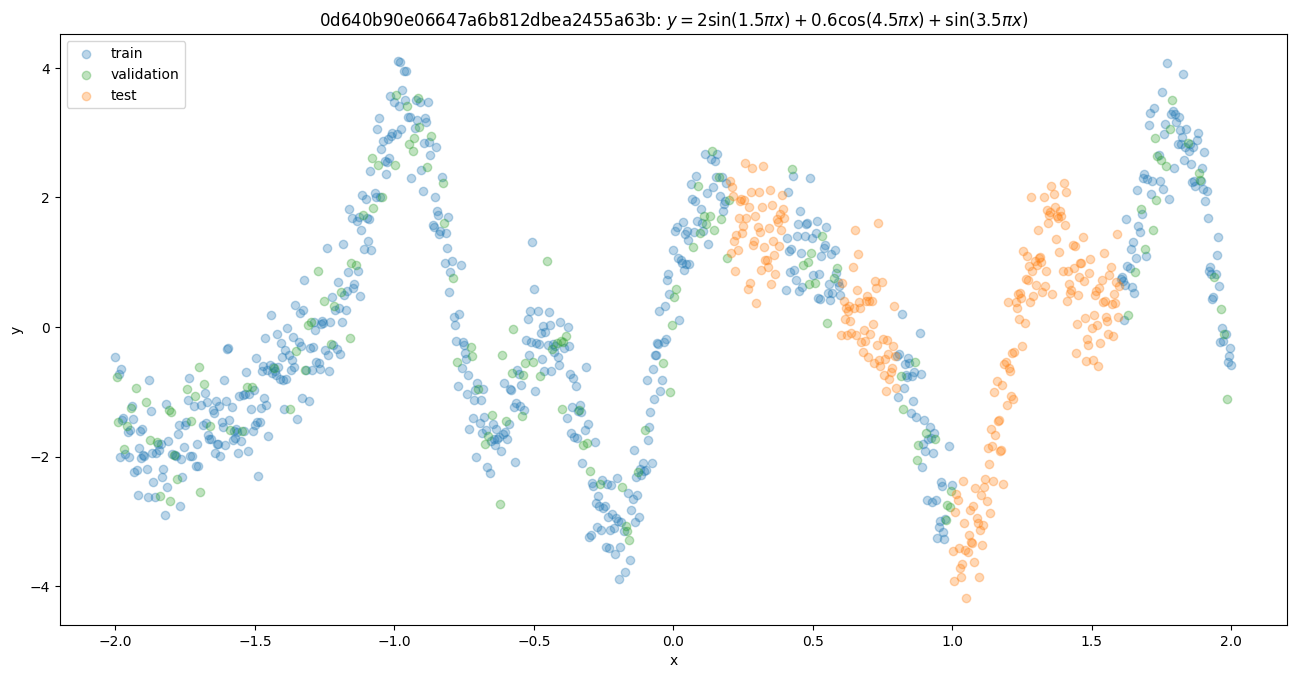
\includegraphics[width=\linewidth]{thesis-report/figures/toy_curves/data/curve3/data.png}
  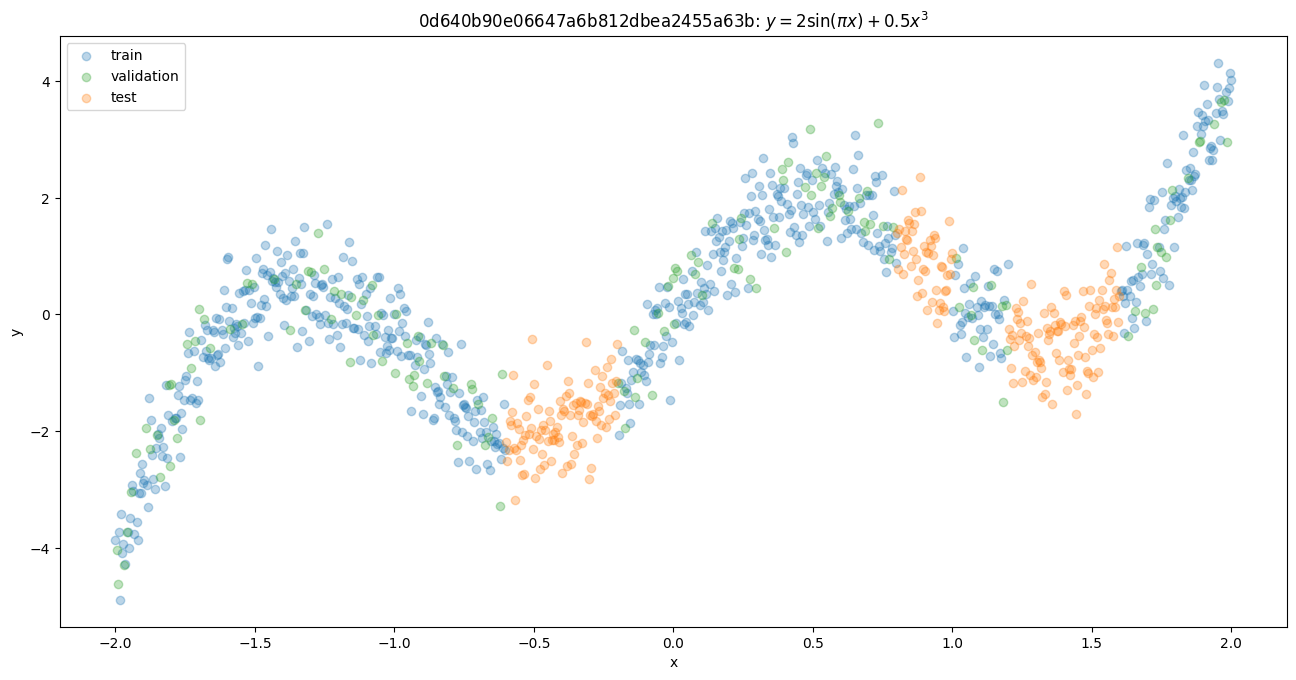
\includegraphics[width=\linewidth]{thesis-report/figures/toy_curves/data/curve5/data.png}
  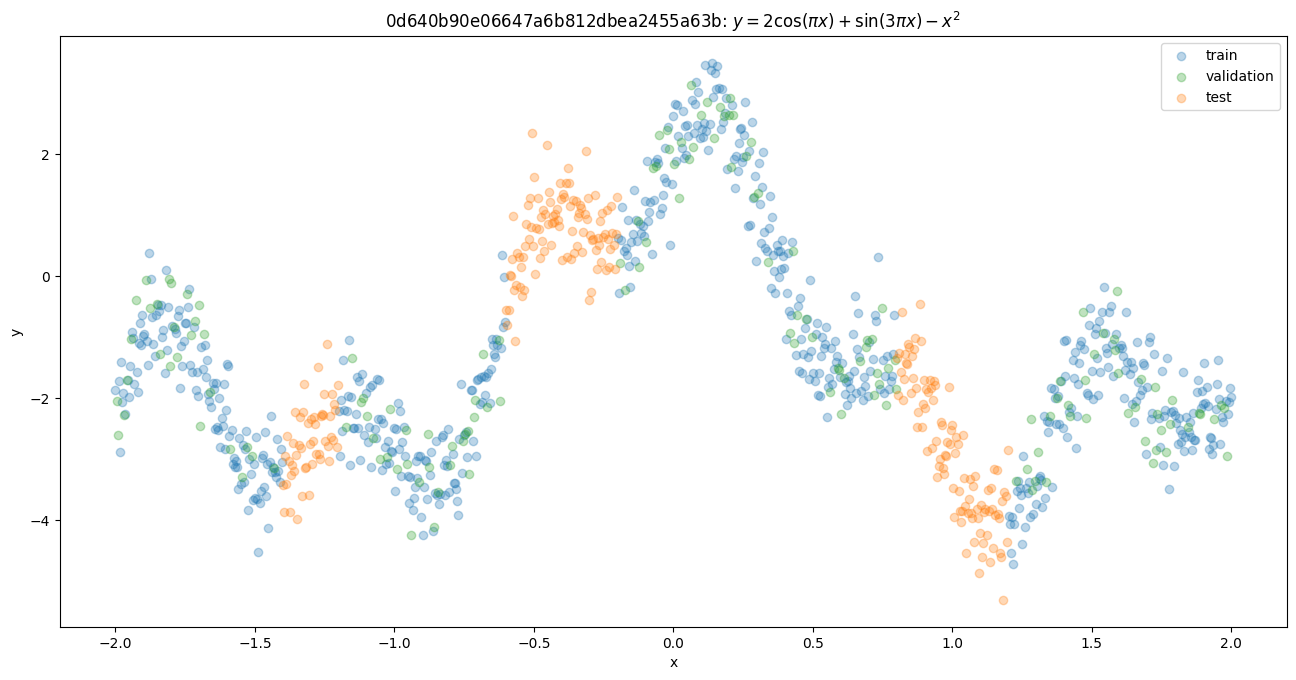
\includegraphics[width=\linewidth]{thesis-report/figures/toy_curves/data/curve7/data.png}
  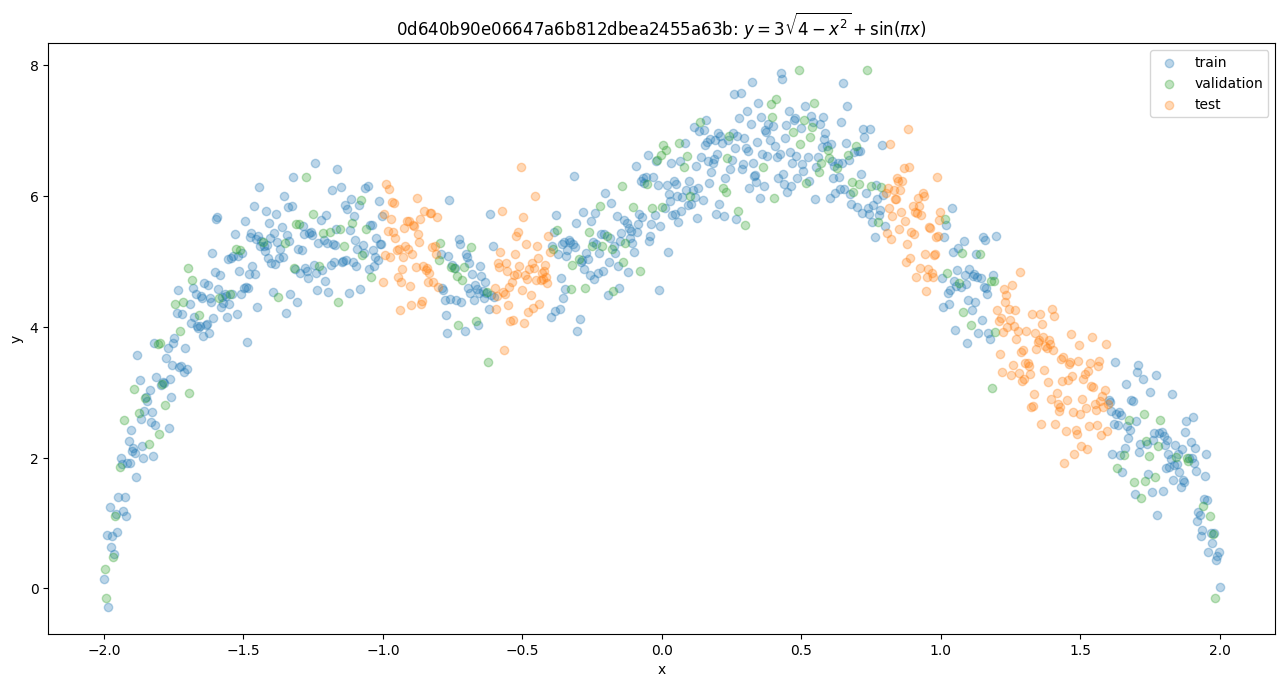
\includegraphics[width=\linewidth]{thesis-report/figures/toy_curves/data/curve9/data.png}
\end{minipage}%
\label{toy-curves}
\caption{All ten Regression Curves}
\end{figure}

\end{document}